% Options for packages loaded elsewhere
% Options for packages loaded elsewhere
\PassOptionsToPackage{unicode}{hyperref}
\PassOptionsToPackage{hyphens}{url}
\PassOptionsToPackage{dvipsnames,svgnames,x11names}{xcolor}
%
\documentclass[
  letterpaper,
  DIV=11,
  numbers=noendperiod]{scrartcl}
\usepackage{xcolor}
\usepackage{amsmath,amssymb}
\setcounter{secnumdepth}{-\maxdimen} % remove section numbering
\usepackage{iftex}
\ifPDFTeX
  \usepackage[T1]{fontenc}
  \usepackage[utf8]{inputenc}
  \usepackage{textcomp} % provide euro and other symbols
\else % if luatex or xetex
  \usepackage{unicode-math} % this also loads fontspec
  \defaultfontfeatures{Scale=MatchLowercase}
  \defaultfontfeatures[\rmfamily]{Ligatures=TeX,Scale=1}
\fi
\usepackage{lmodern}
\ifPDFTeX\else
  % xetex/luatex font selection
\fi
% Use upquote if available, for straight quotes in verbatim environments
\IfFileExists{upquote.sty}{\usepackage{upquote}}{}
\IfFileExists{microtype.sty}{% use microtype if available
  \usepackage[]{microtype}
  \UseMicrotypeSet[protrusion]{basicmath} % disable protrusion for tt fonts
}{}
\makeatletter
\@ifundefined{KOMAClassName}{% if non-KOMA class
  \IfFileExists{parskip.sty}{%
    \usepackage{parskip}
  }{% else
    \setlength{\parindent}{0pt}
    \setlength{\parskip}{6pt plus 2pt minus 1pt}}
}{% if KOMA class
  \KOMAoptions{parskip=half}}
\makeatother
% Make \paragraph and \subparagraph free-standing
\makeatletter
\ifx\paragraph\undefined\else
  \let\oldparagraph\paragraph
  \renewcommand{\paragraph}{
    \@ifstar
      \xxxParagraphStar
      \xxxParagraphNoStar
  }
  \newcommand{\xxxParagraphStar}[1]{\oldparagraph*{#1}\mbox{}}
  \newcommand{\xxxParagraphNoStar}[1]{\oldparagraph{#1}\mbox{}}
\fi
\ifx\subparagraph\undefined\else
  \let\oldsubparagraph\subparagraph
  \renewcommand{\subparagraph}{
    \@ifstar
      \xxxSubParagraphStar
      \xxxSubParagraphNoStar
  }
  \newcommand{\xxxSubParagraphStar}[1]{\oldsubparagraph*{#1}\mbox{}}
  \newcommand{\xxxSubParagraphNoStar}[1]{\oldsubparagraph{#1}\mbox{}}
\fi
\makeatother

\usepackage{color}
\usepackage{fancyvrb}
\newcommand{\VerbBar}{|}
\newcommand{\VERB}{\Verb[commandchars=\\\{\}]}
\DefineVerbatimEnvironment{Highlighting}{Verbatim}{commandchars=\\\{\}}
% Add ',fontsize=\small' for more characters per line
\usepackage{framed}
\definecolor{shadecolor}{RGB}{241,243,245}
\newenvironment{Shaded}{\begin{snugshade}}{\end{snugshade}}
\newcommand{\AlertTok}[1]{\textcolor[rgb]{0.68,0.00,0.00}{#1}}
\newcommand{\AnnotationTok}[1]{\textcolor[rgb]{0.37,0.37,0.37}{#1}}
\newcommand{\AttributeTok}[1]{\textcolor[rgb]{0.40,0.45,0.13}{#1}}
\newcommand{\BaseNTok}[1]{\textcolor[rgb]{0.68,0.00,0.00}{#1}}
\newcommand{\BuiltInTok}[1]{\textcolor[rgb]{0.00,0.23,0.31}{#1}}
\newcommand{\CharTok}[1]{\textcolor[rgb]{0.13,0.47,0.30}{#1}}
\newcommand{\CommentTok}[1]{\textcolor[rgb]{0.37,0.37,0.37}{#1}}
\newcommand{\CommentVarTok}[1]{\textcolor[rgb]{0.37,0.37,0.37}{\textit{#1}}}
\newcommand{\ConstantTok}[1]{\textcolor[rgb]{0.56,0.35,0.01}{#1}}
\newcommand{\ControlFlowTok}[1]{\textcolor[rgb]{0.00,0.23,0.31}{\textbf{#1}}}
\newcommand{\DataTypeTok}[1]{\textcolor[rgb]{0.68,0.00,0.00}{#1}}
\newcommand{\DecValTok}[1]{\textcolor[rgb]{0.68,0.00,0.00}{#1}}
\newcommand{\DocumentationTok}[1]{\textcolor[rgb]{0.37,0.37,0.37}{\textit{#1}}}
\newcommand{\ErrorTok}[1]{\textcolor[rgb]{0.68,0.00,0.00}{#1}}
\newcommand{\ExtensionTok}[1]{\textcolor[rgb]{0.00,0.23,0.31}{#1}}
\newcommand{\FloatTok}[1]{\textcolor[rgb]{0.68,0.00,0.00}{#1}}
\newcommand{\FunctionTok}[1]{\textcolor[rgb]{0.28,0.35,0.67}{#1}}
\newcommand{\ImportTok}[1]{\textcolor[rgb]{0.00,0.46,0.62}{#1}}
\newcommand{\InformationTok}[1]{\textcolor[rgb]{0.37,0.37,0.37}{#1}}
\newcommand{\KeywordTok}[1]{\textcolor[rgb]{0.00,0.23,0.31}{\textbf{#1}}}
\newcommand{\NormalTok}[1]{\textcolor[rgb]{0.00,0.23,0.31}{#1}}
\newcommand{\OperatorTok}[1]{\textcolor[rgb]{0.37,0.37,0.37}{#1}}
\newcommand{\OtherTok}[1]{\textcolor[rgb]{0.00,0.23,0.31}{#1}}
\newcommand{\PreprocessorTok}[1]{\textcolor[rgb]{0.68,0.00,0.00}{#1}}
\newcommand{\RegionMarkerTok}[1]{\textcolor[rgb]{0.00,0.23,0.31}{#1}}
\newcommand{\SpecialCharTok}[1]{\textcolor[rgb]{0.37,0.37,0.37}{#1}}
\newcommand{\SpecialStringTok}[1]{\textcolor[rgb]{0.13,0.47,0.30}{#1}}
\newcommand{\StringTok}[1]{\textcolor[rgb]{0.13,0.47,0.30}{#1}}
\newcommand{\VariableTok}[1]{\textcolor[rgb]{0.07,0.07,0.07}{#1}}
\newcommand{\VerbatimStringTok}[1]{\textcolor[rgb]{0.13,0.47,0.30}{#1}}
\newcommand{\WarningTok}[1]{\textcolor[rgb]{0.37,0.37,0.37}{\textit{#1}}}

\usepackage{longtable,booktabs,array}
\newcounter{none} % for unnumbered tables
\usepackage{calc} % for calculating minipage widths
% Correct order of tables after \paragraph or \subparagraph
\usepackage{etoolbox}
\makeatletter
\patchcmd\longtable{\par}{\if@noskipsec\mbox{}\fi\par}{}{}
\makeatother
% Allow footnotes in longtable head/foot
\IfFileExists{footnotehyper.sty}{\usepackage{footnotehyper}}{\usepackage{footnote}}
\makesavenoteenv{longtable}
\usepackage{graphicx}
\makeatletter
\newsavebox\pandoc@box
\newcommand*\pandocbounded[1]{% scales image to fit in text height/width
  \sbox\pandoc@box{#1}%
  \Gscale@div\@tempa{\textheight}{\dimexpr\ht\pandoc@box+\dp\pandoc@box\relax}%
  \Gscale@div\@tempb{\linewidth}{\wd\pandoc@box}%
  \ifdim\@tempb\p@<\@tempa\p@\let\@tempa\@tempb\fi% select the smaller of both
  \ifdim\@tempa\p@<\p@\scalebox{\@tempa}{\usebox\pandoc@box}%
  \else\usebox{\pandoc@box}%
  \fi%
}
% Set default figure placement to htbp
\def\fps@figure{htbp}
\makeatother


% definitions for citeproc citations
\NewDocumentCommand\citeproctext{}{}
\NewDocumentCommand\citeproc{mm}{%
  \begingroup\def\citeproctext{#2}\cite{#1}\endgroup}
\makeatletter
 % allow citations to break across lines
 \let\@cite@ofmt\@firstofone
 % avoid brackets around text for \cite:
 \def\@biblabel#1{}
 \def\@cite#1#2{{#1\if@tempswa , #2\fi}}
\makeatother
\newlength{\cslhangindent}
\setlength{\cslhangindent}{1.5em}
\newlength{\csllabelwidth}
\setlength{\csllabelwidth}{3em}
\newenvironment{CSLReferences}[2] % #1 hanging-indent, #2 entry-spacing
 {\begin{list}{}{%
  \setlength{\itemindent}{0pt}
  \setlength{\leftmargin}{0pt}
  \setlength{\parsep}{0pt}
  % turn on hanging indent if param 1 is 1
  \ifodd #1
   \setlength{\leftmargin}{\cslhangindent}
   \setlength{\itemindent}{-1\cslhangindent}
  \fi
  % set entry spacing
  \setlength{\itemsep}{#2\baselineskip}}}
 {\end{list}}
\usepackage{calc}
\newcommand{\CSLBlock}[1]{\hfill\break\parbox[t]{\linewidth}{\strut\ignorespaces#1\strut}}
\newcommand{\CSLLeftMargin}[1]{\parbox[t]{\csllabelwidth}{\strut#1\strut}}
\newcommand{\CSLRightInline}[1]{\parbox[t]{\linewidth - \csllabelwidth}{\strut#1\strut}}
\newcommand{\CSLIndent}[1]{\hspace{\cslhangindent}#1}



\setlength{\emergencystretch}{3em} % prevent overfull lines

\providecommand{\tightlist}{%
  \setlength{\itemsep}{0pt}\setlength{\parskip}{0pt}}



 


\usepackage{booktabs}
\usepackage{caption}
\usepackage{longtable}
\usepackage{colortbl}
\usepackage{array}
\usepackage{anyfontsize}
\usepackage{multirow}
\KOMAoption{captions}{tableheading}
\makeatletter
\@ifpackageloaded{tcolorbox}{}{\usepackage[skins,breakable]{tcolorbox}}
\@ifpackageloaded{fontawesome5}{}{\usepackage{fontawesome5}}
\definecolor{quarto-callout-color}{HTML}{909090}
\definecolor{quarto-callout-note-color}{HTML}{0758E5}
\definecolor{quarto-callout-important-color}{HTML}{CC1914}
\definecolor{quarto-callout-warning-color}{HTML}{EB9113}
\definecolor{quarto-callout-tip-color}{HTML}{00A047}
\definecolor{quarto-callout-caution-color}{HTML}{FC5300}
\definecolor{quarto-callout-color-frame}{HTML}{acacac}
\definecolor{quarto-callout-note-color-frame}{HTML}{4582ec}
\definecolor{quarto-callout-important-color-frame}{HTML}{d9534f}
\definecolor{quarto-callout-warning-color-frame}{HTML}{f0ad4e}
\definecolor{quarto-callout-tip-color-frame}{HTML}{02b875}
\definecolor{quarto-callout-caution-color-frame}{HTML}{fd7e14}
\makeatother
\makeatletter
\@ifpackageloaded{caption}{}{\usepackage{caption}}
\AtBeginDocument{%
\ifdefined\contentsname
  \renewcommand*\contentsname{Table of contents}
\else
  \newcommand\contentsname{Table of contents}
\fi
\ifdefined\listfigurename
  \renewcommand*\listfigurename{List of Figures}
\else
  \newcommand\listfigurename{List of Figures}
\fi
\ifdefined\listtablename
  \renewcommand*\listtablename{List of Tables}
\else
  \newcommand\listtablename{List of Tables}
\fi
\ifdefined\figurename
  \renewcommand*\figurename{Figure}
\else
  \newcommand\figurename{Figure}
\fi
\ifdefined\tablename
  \renewcommand*\tablename{Table}
\else
  \newcommand\tablename{Table}
\fi
}
\@ifpackageloaded{float}{}{\usepackage{float}}
\floatstyle{ruled}
\@ifundefined{c@chapter}{\newfloat{codelisting}{h}{lop}}{\newfloat{codelisting}{h}{lop}[chapter]}
\floatname{codelisting}{Listing}
\newcommand*\listoflistings{\listof{codelisting}{List of Listings}}
\makeatother
\makeatletter
\makeatother
\makeatletter
\@ifpackageloaded{caption}{}{\usepackage{caption}}
\@ifpackageloaded{subcaption}{}{\usepackage{subcaption}}
\makeatother
\usepackage{bookmark}
\IfFileExists{xurl.sty}{\usepackage{xurl}}{} % add URL line breaks if available
\urlstyle{same}
% fallback for those not using the hyperref driver hyperxmp:
\makeatletter
\@ifundefined{xmpquote}{\newcommand{\xmpquote}[1]{#1}}{}
\makeatother
\hypersetup{
  pdftitle={Lecture 2: Fund Performance{,} Skill{,} and Luck},
  pdfauthor={Calvin J. Chiou},
  colorlinks=true,
  linkcolor={blue},
  filecolor={Maroon},
  citecolor={Blue},
  urlcolor={Blue},
  pdfcreator={LaTeX via pandoc}}


\title{Lecture 2: Fund Performance, Skill, and Luck}
\usepackage{etoolbox}
\makeatletter
\providecommand{\subtitle}[1]{% add subtitle to \maketitle
  \apptocmd{\@title}{\par {\large #1 \par}}{}{}
}
\makeatother
\subtitle{Institutional Investors}
\author{Calvin J. Chiou}
\date{2026-10-13}
\begin{document}
\maketitle

\renewcommand*\contentsname{Table of contents}
{
\setcounter{tocdepth}{3}
\tableofcontents
}

\subsection{Overview}\label{overview}

Lecture 1 established the \textbf{Carhart four-factor model} as the
standard benchmark for evaluating equity fund performance. A natural
follow-up question is: once we estimate alpha, how do we know whether it
reflects \emph{skill} or simply \emph{luck}?

This lecture digs into three papers on this question:

\begin{itemize}
\tightlist
\item
  \textbf{Fama and French (2010)}: Use bootstrap simulations to separate
  luck from skill in the cross-section of mutual fund alphas. Their
  sobering conclusion: for net returns, few funds have sufficient skill
  to cover their costs.
\item
  \textbf{Berk and van Binsbergen (2015)}: Reframe the question
  entirely. Instead of asking whether alpha is positive, they ask how
  much \emph{dollar value} a fund extracts from markets. Their finding:
  the average fund adds roughly \$3.2 million per year---but competition
  drives net returns to investors toward zero.
\item
  \textbf{Andrikogiannopoulou and Papakonstantinou (2019)}: Ask a prior
  question---\emph{can these tests detect skill even when it is there?}
  They show that the false discovery rate (FDR) methodology, a leading
  alternative to the bootstrap, misclassifies most genuinely skilled
  managers as having zero alpha, because fund returns are too noisy for
  the underlying tests to have power.
\end{itemize}

Together, the first two papers reveal a fundamental tension in the fund
performance literature:

\begin{quote}
\textbf{Skill exists} (Berk \& van Binsbergen), \textbf{but investors
cannot easily capture it} (Fama \& French).
\end{quote}

The third paper adds a methodological warning that cuts across both:

\begin{quote}
\textbf{A finding of ``no skill'' may be a finding about our instruments
rather than about managers.}
\end{quote}

We will:

\begin{enumerate}
\def\labelenumi{\arabic{enumi}.}
\tightlist
\item
  Understand the \textbf{equilibrium accounting} framework for
  evaluating fund performance in aggregate
\item
  Master the \textbf{bootstrap simulation} methodology for
  distinguishing luck from skill
\item
  Examine the \textbf{false discovery rate} approach and why
  (\textbf{andrikogiannopoulou2019?}) argue it fails in this setting
\item
  Learn the \textbf{value-added} measure of skill and why it differs
  from alpha
\item
  Examine the \textbf{Berk-Green (2004)} model and its empirical
  predictions
\item
  Implement a simplified bootstrap exercise in R using CRSP-style mutual
  fund data, and simulate the \textbf{power problem} directly
\end{enumerate}

\begin{center}\rule{0.5\linewidth}{0.5pt}\end{center}

\subsection{1. Motivation: The Luck-vs.-Skill
Problem}\label{motivation-the-luck-vs.-skill-problem}

Suppose you observe a fund with a four-factor alpha of +2\% per year
over 10 years. Should you conclude the manager is skilled? Not
necessarily. With thousands of funds, some will have high alphas purely
by chance. The core challenge is:

\[\underbrace{\hat{\alpha}_i}_{\text{estimated}} = \underbrace{\alpha_i}_{\text{true skill}} + \underbrace{\text{noise}}_{\text{estimation error}}\]

The noise component is not small. The average standard error of a fund's
monthly alpha estimate is about 0.28\% per month (roughly 3.4\%
annualized), as documented by Fama and French (2010). With only 10 years
of data (120 monthly observations), detecting a true annual alpha of 2\%
at the 5\% significance level requires:

\[t = \frac{\hat{\alpha}}{\hat{\sigma}/\sqrt{T}} = \frac{2\%/12}{3.4\%/\sqrt{120}} \approx 0.63\]

This is far below the conventional threshold of 2.0. \textbf{Statistical
power is the central problem} in evaluating individual fund
performance---a point that Wermers (2011) emphasizes and that Lecture 1
introduced.

\begin{tcolorbox}[enhanced jigsaw, arc=.35mm, bottomrule=.15mm, bottomtitle=1mm, breakable, colback=white, colbacktitle=quarto-callout-important-color!10!white, colframe=quarto-callout-important-color-frame, coltitle=black, left=2mm, leftrule=.75mm, opacityback=0, opacitybacktitle=0.6, rightrule=.15mm, title=\textcolor{quarto-callout-important-color}{\faExclamation}\hspace{0.5em}{Important}, titlerule=0mm, toprule=.15mm, toptitle=1mm]

Hold on to this calculation. In Section 4.5 we will see that
(\textbf{andrikogiannopoulou2019?}) build an entire critique of the
modern skill-measurement literature out of exactly this arithmetic. The
low-power problem is not a caveat to be noted and set aside; it can
reverse the economic conclusion.

\end{tcolorbox}

\subsubsection{Two Fundamental
Questions}\label{two-fundamental-questions}

Fama and French (2010) and Berk and Binsbergen (2015) answer
\emph{different} but complementary questions:

\begin{longtable}[]{@{}
  >{\raggedright\arraybackslash}p{(\linewidth - 4\tabcolsep) * \real{0.3333}}
  >{\raggedright\arraybackslash}p{(\linewidth - 4\tabcolsep) * \real{0.3333}}
  >{\raggedright\arraybackslash}p{(\linewidth - 4\tabcolsep) * \real{0.3333}}@{}}
\caption{Two perspectives on fund performance}\tabularnewline
\toprule\noalign{}
\begin{minipage}[b]{\linewidth}\raggedright
Question
\end{minipage} & \begin{minipage}[b]{\linewidth}\raggedright
Fama \& French (2010)
\end{minipage} & \begin{minipage}[b]{\linewidth}\raggedright
Berk \& van Binsbergen (2015)
\end{minipage} \\
\midrule\noalign{}
\endfirsthead
\toprule\noalign{}
\begin{minipage}[b]{\linewidth}\raggedright
Question
\end{minipage} & \begin{minipage}[b]{\linewidth}\raggedright
Fama \& French (2010)
\end{minipage} & \begin{minipage}[b]{\linewidth}\raggedright
Berk \& van Binsbergen (2015)
\end{minipage} \\
\midrule\noalign{}
\endhead
\bottomrule\noalign{}
\endlastfoot
Unit of analysis & Return to investors & Dollar value extracted from
markets \\
Measure of skill & Net / gross alpha & Value added = AUM × gross excess
return \\
Key finding & Few funds cover costs & Average fund adds \$3.2M/year \\
Conclusion on skill & Largely absent (net of fees) & Widespread;
investors recognize it \\
\end{longtable}

\begin{center}\rule{0.5\linewidth}{0.5pt}\end{center}

\subsection{2. Equilibrium Accounting (Fama \& French
2010)}\label{equilibrium-accounting-fama-french-2010}

\subsubsection{2.1 The Zero-Sum Identity}\label{the-zero-sum-identity}

Fama and French (2010) begin with a powerful accounting constraint
called \textbf{equilibrium accounting}. The aggregate of all investors
holds the market portfolio. If passive investors hold passive strategies
with zero alpha, then the aggregate portfolio of \emph{active} investors
must also have zero alpha---before costs.

This is essentially Sharpe's Arithmetic (Sharpe 1991):

\[\underbrace{\alpha_{\text{active, aggregate}}}_{\text{must be zero (before costs)}} = 0\]

After costs:

\[\alpha_{\text{active, aggregate}}^{\text{net}} = -\text{expense ratio} < 0\]

\textbf{Implication}: Active management is a \emph{zero-sum} game before
costs and a \emph{negative-sum} game after costs. If some funds have
positive net alpha, other funds must have an equally large negative net
alpha.

\subsubsection{2.2 Aggregate Portfolio
Results}\label{aggregate-portfolio-results}

Fama and French (2010) estimate regression (1) for the value-weighted
(VW) and equal-weighted (EW) portfolios of all actively managed U.S.
equity mutual funds, 1984--2006:

\[R_{i,t} - R_{f,t} = a_i + b_i(R_{M,t} - R_{f,t}) + s_i \text{SMB}_t + h_i \text{HML}_t + m_i \text{MOM}_t + e_{i,t} \tag{1}\]

Key results from their Table II:

\begin{longtable}[]{@{}llll@{}}
\caption{Aggregate fund performance: net returns (Fama \& French, 2010,
Table II)}\tabularnewline
\toprule\noalign{}
Portfolio & Model & Net α (ann.) & t-stat \\
\midrule\noalign{}
\endfirsthead
\toprule\noalign{}
Portfolio & Model & Net α (ann.) & t-stat \\
\midrule\noalign{}
\endhead
\bottomrule\noalign{}
\endlastfoot
EW & Three-factor & −0.93\% & −2.13 \\
EW & Four-factor & −0.92\% & −2.05 \\
VW & Three-factor & −0.81\% & −2.50 \\
VW & Four-factor & −1.00\% & −3.02 \\
\end{longtable}

The message is clear: \textbf{on net returns, aggregate active
management destroys value by approximately the amount of expense ratios}
(roughly 1\% per year during this period). The VW four-factor alpha of
−1.00\% closely matches the average expense ratio of actively managed
funds.

When returns are measured \emph{gross} (before expense ratios), the
alpha is close to zero:

\begin{longtable}[]{@{}llll@{}}
\caption{Aggregate fund performance: gross returns (Fama \& French,
2010, Table II)}\tabularnewline
\toprule\noalign{}
Portfolio & Model & Gross α (ann.) & t-stat \\
\midrule\noalign{}
\endfirsthead
\toprule\noalign{}
Portfolio & Model & Gross α (ann.) & t-stat \\
\midrule\noalign{}
\endhead
\bottomrule\noalign{}
\endlastfoot
EW & Three-factor & +0.36\% & +0.85 \\
EW & Four-factor & +0.39\% & +0.90 \\
VW & Three-factor & +0.13\% & +0.40 \\
VW & Four-factor & −0.05\% & −0.15 \\
\end{longtable}

The near-zero gross alpha is consistent with equilibrium accounting: in
aggregate, active managers are no better or worse than passive investors
at picking stocks---but they charge fees.

\begin{tcolorbox}[enhanced jigsaw, arc=.35mm, bottomrule=.15mm, bottomtitle=1mm, breakable, colback=white, colbacktitle=quarto-callout-note-color!10!white, colframe=quarto-callout-note-color-frame, coltitle=black, left=2mm, leftrule=.75mm, opacityback=0, opacitybacktitle=0.6, rightrule=.15mm, title=\textcolor{quarto-callout-note-color}{\faInfo}\hspace{0.5em}{Note}, titlerule=0mm, toprule=.15mm, toptitle=1mm]

\textbf{Key insight from equilibrium accounting}: The aggregate results
say nothing about whether \emph{individual} fund managers have skill. It
is possible (and, as we will see, likely) that skilled and unskilled
managers coexist, with the talented ones roughly offsetting the
incompetent ones in aggregate.

\end{tcolorbox}

\begin{center}\rule{0.5\linewidth}{0.5pt}\end{center}

\subsection{3. Bootstrap Simulation
Methodology}\label{bootstrap-simulation-methodology}

The central methodological contribution of Fama and French (2010) is the
\textbf{bootstrap simulation} approach to distinguishing luck from skill
in the cross-section of fund alphas.

\subsubsection{3.1 The Problem with Standard
Inference}\label{the-problem-with-standard-inference}

With thousands of funds, standard t-tests for individual fund alphas are
unreliable for two reasons:

\begin{enumerate}
\def\labelenumi{\arabic{enumi}.}
\tightlist
\item
  \textbf{Multiple comparisons}: With 3,000+ funds, many will have
  extreme alpha estimates purely by chance.
\item
  \textbf{Cross-fund correlation}: Fund returns are correlated (they
  hold similar stocks), so the cross-sectional distribution of
  t-statistics differs from the t-distribution assumed by standard
  tests.
\end{enumerate}

\subsubsection{3.2 The Bootstrap
Procedure}\label{the-bootstrap-procedure}

Fama and French (2010) implement the following procedure:

\textbf{Step 1 --- Demean to impose zero true alpha:}\\
For each fund \(i\), subtract its estimated alpha from its monthly
returns to create ``zero-alpha'' returns:
\[r_{i,t}^* = r_{i,t} - \hat{\alpha}_i\]

\textbf{Step 2 --- Bootstrap:}\\
Draw a random sample (with replacement) of 273 months from the actual
calendar months. Apply the \emph{same} random draw to all funds
simultaneously. This preserves: - The cross-correlation structure of
fund returns - The time-series properties of explanatory returns
(market, SMB, HML, MOM)

\textbf{Step 3 --- Estimate alphas on simulated data:}\\
Run the four-factor regression for each fund on the simulated return
series. Record the t-statistic \(t(\hat{\alpha})\) for each fund.

\textbf{Step 4 --- Repeat 10,000 times:}\\
Build the distribution of \(t(\hat{\alpha})\) under the null hypothesis
of zero true alpha.

\textbf{Step 5 --- Compare:}\\
Compare the actual cross-section of \(t(\hat{\alpha})\) from real fund
data to the simulated distribution. If the actual right tail is
significantly fatter than the simulated right tail, this is evidence of
genuine skill.

\subsubsection{3.3 Why Joint Sampling
Matters}\label{why-joint-sampling-matters}

A crucial feature of the Fama and French (2010) approach is that they
draw the \emph{same} random months for all funds. This is in contrast to
Kosowski et al. (2006), who simulate each fund independently. Joint
sampling matters because:

\begin{itemize}
\tightlist
\item
  It preserves the correlation of alpha estimates across funds
\item
  It captures any correlated heteroskedasticity
\item
  It prevents false evidence of skill that arises from ignoring
  cross-fund dependence
\end{itemize}

Fama and French (2010) show that when Kosowski et al.'s stronger results
are re-examined using joint sampling, the evidence for skill in the
right tail weakens considerably.

\begin{center}\rule{0.5\linewidth}{0.5pt}\end{center}

\subsection{4. Bootstrap Results: Luck
vs.~Skill}\label{bootstrap-results-luck-vs.-skill}

\subsubsection{4.1 Net Returns: Few Managers Cover
Costs}\label{net-returns-few-managers-cover-costs}

Fama and French (2010)'s main result on net returns is sobering. The
cross-section of t(α) estimates from actual fund returns lies almost
entirely to the \emph{left} of the simulated distribution:

\begin{itemize}
\tightlist
\item
  Below the 80th percentile, actual net return t(α) beats the simulated
  values in less than \textbf{1\% of simulation runs}
\item
  Even at the 90th percentile, \textbf{90\% of simulations beat} the
  actual t(α)
\end{itemize}

\textbf{Interpretation}: Most funds do not have sufficient skill to
cover their costs. A fund at the 90th percentile of historical
t(α)---which superficially looks very good---is in fact consistent with
luck, not skill.

The one glimmer of hope: at the \textbf{97th--99th percentiles}, the
actual t(α) estimates are roughly in line with the simulated
distribution. This suggests a small number of truly skilled managers
exist, but they are hidden among lucky underperformers.

\subsubsection{4.2 Gross Returns: Skill Exists, but Is
Modest}\label{gross-returns-skill-exists-but-is-modest}

When returns are measured gross of expenses, evidence of both positive
and negative skill emerges:

\begin{itemize}
\tightlist
\item
  \textbf{Left tail}: Actual t(α) is more extreme than simulated →
  evidence of \emph{truly unskilled} managers who produce negative alpha
  before fees
\item
  \textbf{Right tail}: Actual t(α) exceeds simulated values → evidence
  of \emph{genuinely skilled} managers who outperform passive benchmarks
  before fees
\end{itemize}

Fama and French (2010) quantify the cross-sectional dispersion of true
alpha using additional simulations with \emph{injected} alpha. Their
estimate:

\[\sigma(\alpha^{\text{true}}) \approx 1.25\% \text{ per year}\]

This is a normal distribution with mean zero. Implications:

\begin{itemize}
\tightlist
\item
  Roughly \textbf{16\%} of funds have true gross alpha \textgreater{}
  1.25\% per year (≈10 bp/month)
\item
  Only \textbf{2.4\%} have true gross alpha \textgreater{} 2.50\% per
  year (≈21 bp/month)
\end{itemize}

\begin{tcolorbox}[enhanced jigsaw, arc=.35mm, bottomrule=.15mm, bottomtitle=1mm, breakable, colback=white, colbacktitle=quarto-callout-important-color!10!white, colframe=quarto-callout-important-color-frame, coltitle=black, left=2mm, leftrule=.75mm, opacityback=0, opacitybacktitle=0.6, rightrule=.15mm, title=\textcolor{quarto-callout-important-color}{\faExclamation}\hspace{0.5em}{Important}, titlerule=0mm, toprule=.15mm, toptitle=1mm]

\textbf{The skill that exists is not large enough to cover costs for
most managers.} A true gross alpha of 1.25\% barely covers a 1\% expense
ratio. After fees, most skilled managers produce approximately zero
alpha for investors.

\end{tcolorbox}

\subsubsection{4.3 Graphical Summary: The CDF
Comparison}\label{graphical-summary-the-cdf-comparison}

The key figure in Fama and French (2010) compares the cumulative
distribution functions (CDFs) of actual vs.~simulated t(α):

\begin{itemize}
\tightlist
\item
  For \textbf{net returns}: The actual CDF lies to the \emph{left} of
  the simulated CDF almost everywhere → negative skill overall
\item
  For \textbf{gross returns}: The actual CDF crosses the simulated CDF
  around the 60th--70th percentile → positive skill in the right tail,
  negative skill in the left tail
\end{itemize}

\subsubsection{4.4 A Competing Route: The False Discovery
Rate}\label{a-competing-route-the-false-discovery-rate}

The bootstrap tells us whether the \emph{tails} of the cross-section
look unusual, but it does not directly tell us \emph{what fraction} of
funds have positive, zero, or negative alpha.
(\textbf{barras2010?})---hereafter BSW---propose an approach that does:
the \textbf{false discovery rate} (FDR), imported from the
multiple-testing literature in statistics (\textbf{benjamini1995?}).

The logic is elegant. Run a separate alpha test for every fund and
collect the \(I\) p-values \(\hat{p}_i\). Under the null of zero alpha,
a p-value is uniform on \([0,1]\). So if we pick a high threshold
\(\lambda\)---say 0.5---and assume that \emph{every} p-value above
\(\lambda\) comes from a genuinely zero-alpha fund, we can count those
p-values and extrapolate to the whole interval:

\[\hat{\pi}^0(\lambda) = \frac{\frac{1}{1-\lambda} \cdot \#\{\hat{p}_i : \hat{p}_i > \lambda\}}{I} \tag{2}\]

Knowing \(\hat{\pi}^0\), we can then take the funds that \emph{did}
reject at some significance level \(\gamma\), subtract the number we
expect to have rejected by luck alone (\(\hat{\pi}^0 \cdot \gamma\)),
and recover the proportions of truly negative- and positive-alpha funds:

\[\hat{\pi}^-(\gamma,\lambda) = \frac{\#\{(\hat{\alpha}_i,\hat{p}_i) : \hat{\alpha}_i < 0,\ \hat{p}_i < \gamma\}}{I} - \hat{\pi}^0(\lambda)\cdot\frac{\gamma}{2} \tag{3a}\]

\[\hat{\pi}^+(\gamma,\lambda) = \frac{\#\{(\hat{\alpha}_i,\hat{p}_i) : \hat{\alpha}_i > 0,\ \hat{p}_i < \gamma\}}{I} - \hat{\pi}^0(\lambda)\cdot\frac{\gamma}{2} \tag{3b}\]

Applied to U.S. equity mutual funds, BSW report that \textbf{75\% of
funds have zero alpha net of expenses, 24.4\% have negative alpha, and
only 0.6\% have positive alpha}. These numbers have been enormously
influential. They are read as direct confirmation of Berk and Green
(2004): if almost every fund sits at exactly zero net alpha, that is
what a competitive equilibrium with rational capital reallocation looks
like.

The method spread well beyond mutual funds---to hedge funds, trading
strategies, takeover announcements, and jump detection in asset returns.

\subsubsection{4.5 Reassessing the FDR: Skill, Luck, or Lack of
Power?}\label{reassessing-the-fdr-skill-luck-or-lack-of-power}

(\textbf{andrikogiannopoulou2019?}) ask whether the FDR can actually do
what it claims in this setting. Their answer is no, and the reason is
the arithmetic from Section 1.

Look again at equation (2). It rests on an assumption that is easy to
miss: \emph{every p-value above} \(\lambda\) belongs to a zero-alpha
fund. That holds only if nonzero alphas are large relative to their
standard errors---in other words, only if the individual tests have
\textbf{power}. If a fund has a real alpha of 1\% per year but its alpha
is estimated with a standard error of comparable size, its p-value is
essentially a draw from the uniform distribution too. It lands above
\(\lambda\) roughly as often as a genuinely zero-alpha fund's would, and
the FDR counts it as one.

The bias runs in one direction. Because equation (2) divides by
\(1-\lambda\), each skilled fund that fails to reject contributes
\(1/(1-\lambda) = 2\) funds to the zero-alpha tally when
\(\lambda = 0.5\). \textbf{The FDR systematically overstates the
proportion of zero-alpha funds and understates the proportion with
genuine skill.}

\begin{tcolorbox}[enhanced jigsaw, arc=.35mm, bottomrule=.15mm, bottomtitle=1mm, breakable, colback=white, colbacktitle=quarto-callout-important-color!10!white, colframe=quarto-callout-important-color-frame, coltitle=black, left=2mm, leftrule=.75mm, opacityback=0, opacitybacktitle=0.6, rightrule=.15mm, title=\textcolor{quarto-callout-important-color}{\faExclamation}\hspace{0.5em}{The headline result}, titlerule=0mm, toprule=.15mm, toptitle=1mm]

(\textbf{andrikogiannopoulou2019?}) find that, at the sample sizes
actually available in mutual fund data, the FDR misclassifies as
zero-alpha:

\begin{itemize}
\tightlist
\item
  \textbf{90\%} of funds whose true alpha is ±1\% per year
\item
  \textbf{65\%} of funds whose true alpha is ±2\% per year
\item
  roughly \textbf{30\%} of funds whose true alpha is as large as ±3.5\%
  per year
\end{itemize}

A 2\% annual alpha is not a rounding error. It is roughly twice the
average expense ratio, and a manager who reliably delivered it would be
a star. The methodology cannot see two-thirds of them.

\end{tcolorbox}

\paragraph{Why BSW's own simulation looked so
convincing}\label{why-bsws-own-simulation-looked-so-convincing}

BSW validated the FDR with a simulation, and in that simulation it
performed beautifully. (\textbf{andrikogiannopoulou2019?}) show why: the
simulation was run under conditions far more favorable than the real
data.

\begin{longtable}[]{@{}
  >{\raggedright\arraybackslash}p{(\linewidth - 2\tabcolsep) * \real{0.5000}}
  >{\raggedright\arraybackslash}p{(\linewidth - 2\tabcolsep) * \real{0.5000}}@{}}
\caption{Why the BSW simulation overstates FDR accuracy}\tabularnewline
\toprule\noalign{}
\begin{minipage}[b]{\linewidth}\raggedright
BSW simulation assumption
\end{minipage} & \begin{minipage}[b]{\linewidth}\raggedright
Reality in mutual fund data
\end{minipage} \\
\midrule\noalign{}
\endfirsthead
\toprule\noalign{}
\begin{minipage}[b]{\linewidth}\raggedright
BSW simulation assumption
\end{minipage} & \begin{minipage}[b]{\linewidth}\raggedright
Reality in mutual fund data
\end{minipage} \\
\midrule\noalign{}
\endhead
\bottomrule\noalign{}
\endlastfoot
Nonzero alphas at −3.2\% and +3.8\% per year & Large share of funds have
alphas between 1\% and 2.5\% \\
\(T = 384\) months per fund (the \emph{maximum} in the data) & Median
150, mean 180 observations per fund \\
\(N = 1{,}400\) funds, balanced panel & 2,076 funds, unbalanced panel \\
Little or no cross-sectional error correlation & Substantial correlation
from common strategies \\
\end{longtable}

Each of these pushes in the same direction. The result is that a
methodology which looks nearly unbiased in its original validation
becomes badly biased once the data-generating process resembles the data
it is applied to.

\paragraph{Three findings that make this hard to
fix}\label{three-findings-that-make-this-hard-to-fix}

\textbf{More funds do not help.} This is the most counterintuitive
result. Increasing \(N\) leaves the bias essentially unchanged, because
\(N\) affects neither the power of each individual test nor the
distribution of p-values. (\textbf{andrikogiannopoulou2019?}) put it
memorably: it is like estimating a population's mean weight by weighing
more and more people on a biased scale. Only \(T\)---observations per
fund---matters, and convergence is glacial. They find that \textbf{even
200 years of monthly data would not be enough} to get accurate estimates
for realistic alpha distributions.

\textbf{Confidence intervals are not a safety net.} For roughly half the
data-generating processes they examine, the nominal 95\% confidence
intervals around the FDR estimates \textbf{never} contain the true
proportions across 1,000 simulated samples. Realistic cross-sectional
correlation in residuals inflates the estimator's variability by about a
factor of five, widening 90\% intervals by 4.6 to 7.5 times.

\textbf{The correction may not beat no correction.} For alphas of 1\% or
2\% per year, the FDR does not outperform the naive ``no-luck'' approach
of simply counting significant alphas without any multiple-testing
adjustment---and can do worse, because its bias is so large.

\paragraph{The connection back to Fama and
French}\label{the-connection-back-to-fama-and-french}

There is a result here that speaks directly to Section 4.2. Recall that
Fama and French (2010) estimate the cross-sectional dispersion of true
alpha at about 1.25\% per year. (\textbf{andrikogiannopoulou2019?})
simulate a data-generating process calibrated close to that
estimate---alphas drawn from a normal with \(\sigma_\alpha = 1.5\%\),
with only \textbf{1\%} of funds having exactly zero alpha---and apply
the FDR to it. The FDR reports that \textbf{70\%} of funds have zero
alpha.

In other words: take the world that Fama and French's own estimates
describe, and the FDR will tell you it is the world that BSW found.

\begin{tcolorbox}[enhanced jigsaw, arc=.35mm, bottomrule=.15mm, bottomtitle=1mm, breakable, colback=white, colbacktitle=quarto-callout-note-color!10!white, colframe=quarto-callout-note-color-frame, coltitle=black, left=2mm, leftrule=.75mm, opacityback=0, opacitybacktitle=0.6, rightrule=.15mm, title=\textcolor{quarto-callout-note-color}{\faInfo}\hspace{0.5em}{What this does and does not overturn}, titlerule=0mm, toprule=.15mm, toptitle=1mm]

(\textbf{andrikogiannopoulou2019?}) is a critique of a
\textbf{methodology}, not a claim that mutual fund managers are secretly
skilled. They do not estimate skill themselves in this paper. What they
establish is that the widely cited ``75\% of funds have zero alpha''
figure cannot bear the economic weight placed on it---in particular, it
is not evidence for the Berk and Green (2004) equilibrium, because an
estimator with this much bias would report approximately that number
whether or not Berk-Green were true.

A test that returns the same answer under the hypothesis and its
negation is not evidence about the hypothesis.

\end{tcolorbox}

\paragraph{What to do instead}\label{what-to-do-instead}

The authors are constructive. Their recommendations:

\begin{enumerate}
\def\labelenumi{\arabic{enumi}.}
\tightlist
\item
  \textbf{Check power before trusting the estimator.} Simulate your own
  data-generating process and verify that individual tests have enough
  power for the FDR's assumptions to hold. This is cheap---we do it in
  Section 10.
\item
  \textbf{Pool cross-sectional information} rather than testing each
  fund in isolation. Approaches that estimate the whole cross-sectional
  distribution of alpha, rather than running \(I\) separate underpowered
  tests, extract far more from the same data. They point to
  (\textbf{harvey2018?}) and their own related work in this vein.
\item
  \textbf{Be wary of the FDR wherever the signal-to-noise ratio is low.}
  The problem is not specific to mutual funds. Any application with
  large \(N\) and small \(T\)---hedge funds, trading strategies, event
  studies---inherits it.
\end{enumerate}

\begin{center}\rule{0.5\linewidth}{0.5pt}\end{center}

\subsection{5. The Value-Added Approach (Berk \& van Binsbergen
2015)}\label{the-value-added-approach-berk-van-binsbergen-2015}

\subsubsection{5.1 Why Alpha Fails as a Skill
Measure}\label{why-alpha-fails-as-a-skill-measure}

Berk and Binsbergen (2015) make a fundamental theoretical point:
\textbf{neither net alpha nor gross alpha correctly measures managerial
skill}. The argument proceeds as follows.

Under standard neoclassical assumptions (rational investors, competitive
markets, optimizing managers with decreasing returns to scale):

\textbf{Net alpha} measures market efficiency, not skill. If investors
are rational and markets competitive, the net alpha is driven to zero by
capital flows---regardless of skill. A fund with high skill attracts
capital until its net alpha is competed away.

\textbf{Gross alpha} equals the fee the manager charges. To see this,
note:
\[\alpha^{\text{gross}} = \alpha^{\text{net}} + f_i = 0 + f_i = f_i\]

where \(f_i\) is the fund's percentage fee. The gross alpha is a
\emph{choice variable} of the manager, not a measure of skill. A manager
who indexes more of the portfolio can achieve any desired gross alpha by
adjusting the fee accordingly.

This leads to a striking \textbf{proposition} (Berk \& van Binsbergen
2015, Proposition 1):

\begin{quote}
\emph{The only condition under which gross alpha measures managerial
skill is if all managers set their fees to ensure that the AUM of all
funds is exactly \$1.}
\end{quote}

Since AUM varies enormously across funds, gross alpha is an unreliable
proxy for skill in practice (their Table 8: cross-sectional correlation
between value added and gross alpha is only 23\%, with \(R^2 = 5\%\)).

\subsubsection{5.2 The Value-Added
Measure}\label{the-value-added-measure}

The correct measure of managerial skill, according to Berk and
Binsbergen (2015), is the \textbf{value added} of the fund---the dollar
value extracted from financial markets:

\[V_{i,t} = q_{i,t-1} \cdot (R_{i,t}^g - R_{i,t}^B) \tag{4}\]

where: - \(q_{i,t-1}\) = assets under management (AUM) at the end of the
prior period - \(R_{i,t}^g\) = gross excess return of fund \(i\) at time
\(t\) - \(R_{i,t}^B\) = benchmark return (the investor's next best
alternative)

The fund's \textbf{skill} is the time-series expectation of value added:
\[S_i \equiv \mathbb{E}[V_{i,t}] \tag{5}\]

Intuitively: a manager who adds 1\% alpha on a \$10 billion fund adds
\emph{more value} (\$100 million) than a manager who adds 10\% alpha on
a \$1 million fund (\$100,000), even though the former has a much lower
gross alpha.

\begin{tcolorbox}[enhanced jigsaw, arc=.35mm, bottomrule=.15mm, bottomtitle=1mm, breakable, colback=white, colbacktitle=quarto-callout-tip-color!10!white, colframe=quarto-callout-tip-color-frame, coltitle=black, left=2mm, leftrule=.75mm, opacityback=0, opacitybacktitle=0.6, rightrule=.15mm, title=\textcolor{quarto-callout-tip-color}{\faLightbulb}\hspace{0.5em}{Tip}, titlerule=0mm, toprule=.15mm, toptitle=1mm]

Notice that the value-added measure sidesteps part of the problem
(\textbf{andrikogiannopoulou2019?}) identify. Dollar value added is
estimated from the \emph{level} of AUM times realized excess return, and
its cross-sectional dispersion is enormous, so the signal-to-noise ratio
is far better than it is for percentage alpha. This is one reason Berk
and Binsbergen (2015) can document persistence over ten years where
alpha-based studies find almost none.

\end{tcolorbox}

\subsubsection{5.3 The Benchmark: Vanguard Index
Funds}\label{the-benchmark-vanguard-index-funds}

A critical design choice in Berk and Binsbergen (2015) is the
\textbf{benchmark}. The standard approach (Carhart four factors) uses
factor-mimicking portfolios that:

\begin{enumerate}
\def\labelenumi{\arabic{enumi}.}
\tightlist
\item
  Were not actually available to investors in the early part of the
  sample (e.g., small-cap and value index funds were not widely
  available until the early 1990s)
\item
  Do not account for transaction costs
\item
  May contain hindsight bias
\end{enumerate}

Berk and Binsbergen (2015) instead use \textbf{Vanguard index funds} as
the benchmark---the actual investment opportunity available to investors
at each point in time. This benchmark:

\begin{itemize}
\tightlist
\item
  Is guaranteed to be tradable and marketed
\item
  Includes transaction costs
\item
  Reflects the dynamic evolution of available passive strategies
\end{itemize}

The FFC (Fama-French-Carhart) factor portfolios themselves produce
significantly positive alpha relative to Vanguard benchmarks:

\begin{longtable}[]{@{}llll@{}}
\caption{Net alpha of FFC factor portfolios vs.~Vanguard benchmark (Berk
\& van Binsbergen 2015, Table 2)}\tabularnewline
\toprule\noalign{}
Factor & Alpha (bp/month) & t-stat & Adjusted \(R^2\) \\
\midrule\noalign{}
\endfirsthead
\toprule\noalign{}
Factor & Alpha (bp/month) & t-stat & Adjusted \(R^2\) \\
\midrule\noalign{}
\endhead
\bottomrule\noalign{}
\endlastfoot
Market & 2 & 0.83 & 99\% \\
SMB & 22 & 2.80 & 74\% \\
HML & 35 & 3.37 & 52\% \\
UMD & 70 & 3.38 & 15\% \\
\end{longtable}

The high alphas of SMB, HML, and UMD reflect the hindsight bias embedded
in using these factors: investors in the early sample period could not
cheaply access these strategies.

\begin{center}\rule{0.5\linewidth}{0.5pt}\end{center}

\subsection{6. The Berk-Green (2004)
Model}\label{the-berk-green-2004-model}

Both papers reference the theoretical framework of Berk and Green
(2004), which provides an equilibrium model of the mutual fund industry.
The key predictions of the model:

\begin{enumerate}
\def\labelenumi{\arabic{enumi}.}
\tightlist
\item
  \textbf{Fund managers have skill} (positive gross alpha on the first
  dollar managed)
\item
  \textbf{Decreasing returns to scale}: the more capital a manager
  actively manages, the lower the alpha per dollar
\item
  \textbf{Rational investors}: capital flows to funds with positive
  expected alpha until expected net alpha is driven to zero
\item
  \textbf{In equilibrium}: every fund has zero net alpha, but managers
  capture all economic rents through fees
\end{enumerate}

This model has three testable predictions that the papers address:

\begin{longtable}[]{@{}
  >{\raggedright\arraybackslash}p{(\linewidth - 6\tabcolsep) * \real{0.2500}}
  >{\raggedright\arraybackslash}p{(\linewidth - 6\tabcolsep) * \real{0.2500}}
  >{\raggedright\arraybackslash}p{(\linewidth - 6\tabcolsep) * \real{0.2500}}
  >{\raggedright\arraybackslash}p{(\linewidth - 6\tabcolsep) * \real{0.2500}}@{}}
\caption{Testing the Berk-Green (2004) model}\tabularnewline
\toprule\noalign{}
\begin{minipage}[b]{\linewidth}\raggedright
Prediction
\end{minipage} & \begin{minipage}[b]{\linewidth}\raggedright
Fama \& French (2010)
\end{minipage} & \begin{minipage}[b]{\linewidth}\raggedright
Berk \& van Binsbergen (2015)
\end{minipage} & \begin{minipage}[b]{\linewidth}\raggedright
Andrikogiannopoulou \& Papakonstantinou (2019)
\end{minipage} \\
\midrule\noalign{}
\endfirsthead
\toprule\noalign{}
\begin{minipage}[b]{\linewidth}\raggedright
Prediction
\end{minipage} & \begin{minipage}[b]{\linewidth}\raggedright
Fama \& French (2010)
\end{minipage} & \begin{minipage}[b]{\linewidth}\raggedright
Berk \& van Binsbergen (2015)
\end{minipage} & \begin{minipage}[b]{\linewidth}\raggedright
Andrikogiannopoulou \& Papakonstantinou (2019)
\end{minipage} \\
\midrule\noalign{}
\endhead
\bottomrule\noalign{}
\endlastfoot
Zero net alpha in aggregate & \textbf{Rejected}: aggregate net alpha ≈
−1\%/year & Not directly tested; focus on value added & Not tested
directly \\
Investors identify and reward skill & Not examined & \textbf{Confirmed}:
current compensation predicts future value added & Not examined \\
Most individual funds have zero alpha & Consistent with bootstrap
evidence & Not the right question & \textbf{Cannot be inferred from FDR
estimates}: the estimator would report this regardless \\
\end{longtable}

Fama and French (2010) explicitly state that their results ``reject most
of {[}Berk and Green's{]} predictions about mutual fund returns.'' The
aggregate negative net alpha contradicts the model's prediction that all
managers have zero expected net alpha in equilibrium.

Berk and Binsbergen (2015) find results more consistent with Berk-Green:
investors \emph{do} appear to identify skilled managers (compensation
predicts future value added), and the cross-sectional distribution of
skill is persistent for up to ten years.

(\textbf{andrikogiannopoulou2019?}) add a third position that is neither
support nor rejection: the FDR evidence most often cited \emph{in favor}
of Berk-Green is uninformative about it, so the model's empirical status
rests on the other two literatures rather than on the ``75\% zero
alpha'' statistic.

\begin{center}\rule{0.5\linewidth}{0.5pt}\end{center}

\subsection{7. Key Results: Berk \& van Binsbergen
(2015)}\label{key-results-berk-van-binsbergen-2015}

\subsubsection{7.1 Average Fund Adds Positive
Value}\label{average-fund-adds-positive-value}

Using the Vanguard benchmark, the \textbf{average mutual fund adds
approximately \$3.2 million per year} (time-weighted mean:
\$270,000/month in Y2000 dollars). The t-statistic is 5.74---strong
statistical evidence against the no-skill hypothesis.

Using the FFC risk adjustment, the result is similar: \$250,000/month, t
= 3.94.

However, the distribution is highly skewed:

\begin{longtable}[]{@{}ll@{}}
\caption{Distribution of value added across funds (Berk \& van
Binsbergen 2015, Table 3)}\tabularnewline
\toprule\noalign{}
Percentile & Value Added (Y2000 \$/month) \\
\midrule\noalign{}
\endfirsthead
\toprule\noalign{}
Percentile & Value Added (Y2000 \$/month) \\
\midrule\noalign{}
\endhead
\bottomrule\noalign{}
\endlastfoot
1st & −\$3.60M \\
10th & −\$590K \\
50th (median) & −\$20K \\
90th & +\$750K \\
99th & +\$7.82M \\
\% with positive value added & 43\% \\
\end{longtable}

Most funds destroy value; the \emph{average} is positive because the
minority of skilled managers manages most of the capital.

\subsubsection{7.2 Persistence of Value
Added}\label{persistence-of-value-added}

The most compelling evidence for skill is the \textbf{persistence} of
value added for up to 10 years. Berk and Binsbergen (2015) construct a
non-parametric test: do funds in the top decile (by skill ratio)
continue to beat funds in the bottom decile in future periods?

The null hypothesis is Binomial(n, ½): under no skill, top decile funds
beat bottom decile funds 50\% of the time. The actual results:

\begin{itemize}
\tightlist
\item
  Top decile beats bottom decile at every horizon from 3 to 10 years
\item
  The null is rejected at the 95\% confidence level at most horizons
\item
  The top decile controls approximately 25\% of total AUM (investors
  reward skill with capital)
\end{itemize}

This persistence is far longer than anything documented using alpha
measures, which Carhart (1997) and others have found to be largely
unpredictable.

\subsubsection{7.3 Investors Can Identify
Skill}\label{investors-can-identify-skill}

A surprising finding: \textbf{current managerial compensation predicts
future value added better than past value added does.} This means
investors are not ``dumb money'' chasing past returns---they appear to
genuinely infer managerial skill and allocate capital accordingly.

Managerial compensation = AUM × fee rate. Since fee rates vary little
across funds, it is primarily investors' capital allocation decisions
that determine compensation. The finding implies that the
flow-performance relationship reflects rational information processing,
consistent with Berk and Green (2004).

\subsubsection{7.4 Where Does the Value
Go?}\label{where-does-the-value-go}

Value added can be decomposed into:

\[V_{i,t} = \underbrace{q_{i,t-1} \cdot f_{i,t-1}}_{\text{fees (compensation)}} + \underbrace{q_{i,t-1} \cdot \varepsilon_{i,t}}_{\text{returns to investors}}\]

Berk and Binsbergen (2015) find that \textbf{the net alpha to investors
is approximately zero}---managers capture essentially all economic rents
through fees. Investors receive no abnormal return from investing in
skilled funds because competition drives net alpha to zero. This is the
central prediction of Berk and Green (2004), and it is confirmed by the
data.

Furthermore, roughly \textbf{half of total value added comes from
diversification services} (the value Vanguard itself charges for) and
half from active stock picking and market timing.

\begin{center}\rule{0.5\linewidth}{0.5pt}\end{center}

\subsection{8. Reconciling the Three
Papers}\label{reconciling-the-three-papers}

A reader might be confused: Fama \& French say skill is rare; Berk \&
van Binsbergen say the average fund is skilled; Andrikogiannopoulou \&
Papakonstantinou say we may not be able to tell. Who is right?

All three are right---they are answering different questions:

\begin{longtable}[]{@{}
  >{\raggedright\arraybackslash}p{(\linewidth - 6\tabcolsep) * \real{0.2500}}
  >{\raggedright\arraybackslash}p{(\linewidth - 6\tabcolsep) * \real{0.2500}}
  >{\raggedright\arraybackslash}p{(\linewidth - 6\tabcolsep) * \real{0.2500}}
  >{\raggedright\arraybackslash}p{(\linewidth - 6\tabcolsep) * \real{0.2500}}@{}}
\caption{Reconciling the three papers}\tabularnewline
\toprule\noalign{}
\begin{minipage}[b]{\linewidth}\raggedright
Dimension
\end{minipage} & \begin{minipage}[b]{\linewidth}\raggedright
Fama \& French (2010)
\end{minipage} & \begin{minipage}[b]{\linewidth}\raggedright
Berk \& van Binsbergen (2015)
\end{minipage} & \begin{minipage}[b]{\linewidth}\raggedright
Andrikogiannopoulou \& Papakonstantinou (2019)
\end{minipage} \\
\midrule\noalign{}
\endfirsthead
\toprule\noalign{}
\begin{minipage}[b]{\linewidth}\raggedright
Dimension
\end{minipage} & \begin{minipage}[b]{\linewidth}\raggedright
Fama \& French (2010)
\end{minipage} & \begin{minipage}[b]{\linewidth}\raggedright
Berk \& van Binsbergen (2015)
\end{minipage} & \begin{minipage}[b]{\linewidth}\raggedright
Andrikogiannopoulou \& Papakonstantinou (2019)
\end{minipage} \\
\midrule\noalign{}
\endhead
\bottomrule\noalign{}
\endlastfoot
Skill exists? & Modest evidence (gross returns only) & Yes---average
fund adds \$3.2M/year & Unanswerable from FDR estimates \\
Do investors benefit? & No---net returns are negative & No---net alpha ≈
0 (rents captured by managers) & Not addressed \\
Can investors identify skilled funds? & Not examined &
Yes---compensation predicts future value added & Not addressed \\
Right benchmark? & FFC factors & Vanguard index funds (preferred) & Not
addressed \\
Can the \emph{test} detect skill? & Bootstrap has some power in the
tails & Value added has far better signal-to-noise & \textbf{No}---FDR
misses 65\% of ±2\% alphas \\
\end{longtable}

The substantive resolution between the first two:

\begin{quote}
\textbf{Skill exists and is measurable in dollars. But competition among
investors drives the net return to investors to zero. Skilled managers
capture all rents through fees and fund size. The \emph{dollar} evidence
of skill is clear; the \emph{return} evidence is weak because rational
flows eliminate the return opportunity.}
\end{quote}

And the methodological caution the third paper adds:

\begin{quote}
\textbf{Before interpreting any ``no skill'' finding, ask what the test
would have reported had skill been present. If the answer is ``the same
thing,'' the finding is about the test.}
\end{quote}

\begin{center}\rule{0.5\linewidth}{0.5pt}\end{center}

\subsection{9. Implications for
Practice}\label{implications-for-practice}

\subsubsection{9.1 For Performance
Evaluation}\label{for-performance-evaluation}

\begin{enumerate}
\def\labelenumi{\arabic{enumi}.}
\item
  \textbf{Do not rely on alpha alone.} The cross-section of alpha
  estimates is dominated by noise. Only the extreme tails (99th
  percentile and beyond) provide any reliable signal of genuine skill
  after accounting for multiple comparisons.
\item
  \textbf{Consider fund size.} Berk \& van Binsbergen demonstrate that
  small funds can have high alpha but low value added. A large fund with
  modest alpha may be adding more value in dollar terms.
\item
  \textbf{Use the right benchmark.} FFC factors contain hindsight bias.
  Traded alternatives (passive index funds) are a more appropriate
  benchmark for evaluating whether a manager beats the investor's actual
  opportunity set.
\end{enumerate}

\subsubsection{9.2 For Investors}\label{for-investors}

\begin{enumerate}
\def\labelenumi{\arabic{enumi}.}
\setcounter{enumi}{3}
\item
  \textbf{The expected net return from active management is
  approximately zero or slightly negative.} Fama \& French's equilibrium
  accounting tells us this must be true on average. The zero or negative
  net alpha is not a measurement artifact.
\item
  \textbf{Identifying skilled managers is difficult but not impossible.}
  Berk \& van Binsbergen show that investors in aggregate appear to do
  so (compensation predicts performance). But individual investors face
  a severe information disadvantage relative to the institutional
  investors who dominate capital flows.
\item
  \textbf{Passive investing dominates for most investors.} Even if skill
  exists and is persistent, skilled managers capture their own rents.
  Net alpha to investors is approximately zero for the best funds---and
  negative for most funds.
\end{enumerate}

\subsubsection{9.3 For Research}\label{for-research}

\begin{enumerate}
\def\labelenumi{\arabic{enumi}.}
\setcounter{enumi}{6}
\item
  \textbf{Bootstrap simulation is the gold standard} for detecting skill
  in cross-sections of fund returns. Standard t-tests are inadequate due
  to multiple comparisons and cross-fund correlation.
\item
  \textbf{Statistical power is severely limited} with typical mutual
  fund sample sizes. A fund needs decades of monthly data to reliably
  distinguish a 2\% annual alpha from noise. For shorter-lived funds,
  inference requires simulation-based methods.
\item
  \textbf{Validate your estimator on a realistic DGP, not a convenient
  one} (\textbf{andrikogiannopoulou2019?}). BSW's validation simulation
  was internally correct; it simply assumed alphas far larger and panels
  far longer than the data contain. Before adopting any estimator,
  simulate it under parameters calibrated to the data you actually have.
\item
  \textbf{Adding observations in the cross-section does not fix a power
  problem.} Power depends on \(T\) per unit, not \(N\). This is worth
  internalizing: it applies to panel settings throughout empirical
  finance, not just fund performance.
\end{enumerate}

\begin{center}\rule{0.5\linewidth}{0.5pt}\end{center}

\subsection{10. Empirical
Implementation}\label{empirical-implementation}

In this section we implement a simplified version of the Fama and French
(2010) bootstrap procedure. We use the same 10 US ETFs and factor data
from Lecture 1 to illustrate the methodology. Note that this exercise is
pedagogical---the full Fama and French (2010) analysis uses thousands of
actively managed mutual funds.

\subsubsection{Setup}\label{setup}

\begin{Shaded}
\begin{Highlighting}[]
\FunctionTok{library}\NormalTok{(tidyverse)}
\FunctionTok{library}\NormalTok{(tidyquant)}
\FunctionTok{library}\NormalTok{(frenchdata)}
\FunctionTok{library}\NormalTok{(broom)}
\FunctionTok{library}\NormalTok{(gt)}
\FunctionTok{library}\NormalTok{(scales)}

\FunctionTok{set.seed}\NormalTok{(}\DecValTok{42}\NormalTok{)  }\CommentTok{\# reproducibility}
\end{Highlighting}
\end{Shaded}

\subsubsection{Load Data from Lecture 1}\label{load-data-from-lecture-1}

\begin{Shaded}
\begin{Highlighting}[]
\CommentTok{\# {-}{-}{-} ETF list and labels {-}{-}{-}}
\NormalTok{etf\_tickers }\OtherTok{\textless{}{-}} \FunctionTok{c}\NormalTok{(}\StringTok{"SPY"}\NormalTok{,}\StringTok{"QQQ"}\NormalTok{,}\StringTok{"IWM"}\NormalTok{,}\StringTok{"VTV"}\NormalTok{,}\StringTok{"VUG"}\NormalTok{,}\StringTok{"ARKK"}\NormalTok{,}\StringTok{"XLE"}\NormalTok{,}\StringTok{"XLF"}\NormalTok{,}\StringTok{"VNQ"}\NormalTok{,}\StringTok{"IWD"}\NormalTok{)}
\NormalTok{etf\_labels  }\OtherTok{\textless{}{-}} \FunctionTok{tibble}\NormalTok{(}
  \AttributeTok{symbol   =}\NormalTok{ etf\_tickers,}
  \AttributeTok{name     =} \FunctionTok{c}\NormalTok{(}\StringTok{"S\&P 500"}\NormalTok{,}\StringTok{"Nasdaq{-}100"}\NormalTok{,}\StringTok{"Russell 2000"}\NormalTok{,}\StringTok{"Vanguard Value"}\NormalTok{,}
               \StringTok{"Vanguard Growth"}\NormalTok{,}\StringTok{"ARK Innovation"}\NormalTok{,}\StringTok{"Energy Sector"}\NormalTok{,}
               \StringTok{"Financials Sector"}\NormalTok{,}\StringTok{"Real Estate (REIT)"}\NormalTok{,}\StringTok{"Russell 1000 Value"}\NormalTok{),}
  \AttributeTok{category =} \FunctionTok{c}\NormalTok{(}\StringTok{"Broad market"}\NormalTok{,}\StringTok{"Tech/Growth"}\NormalTok{,}\StringTok{"Small cap"}\NormalTok{,}\StringTok{"Large value"}\NormalTok{,}
               \StringTok{"Large growth"}\NormalTok{,}\StringTok{"Active growth"}\NormalTok{,}\StringTok{"Sector"}\NormalTok{,}\StringTok{"Sector"}\NormalTok{,}\StringTok{"REIT"}\NormalTok{,}\StringTok{"Large value"}\NormalTok{)}
\NormalTok{)}

\CommentTok{\# {-}{-}{-} Download prices {-}{-}{-}}
\NormalTok{start\_date }\OtherTok{\textless{}{-}} \StringTok{"2015{-}01{-}01"}
\NormalTok{end\_date   }\OtherTok{\textless{}{-}} \StringTok{"2024{-}12{-}31"}

\NormalTok{prices\_raw }\OtherTok{\textless{}{-}} \FunctionTok{tq\_get}\NormalTok{(etf\_tickers, }\AttributeTok{from =}\NormalTok{ start\_date, }\AttributeTok{to =}\NormalTok{ end\_date,}
                     \AttributeTok{get =} \StringTok{"stock.prices"}\NormalTok{)}

\CommentTok{\# {-}{-}{-} Monthly returns {-}{-}{-}}
\NormalTok{returns\_monthly }\OtherTok{\textless{}{-}}\NormalTok{ prices\_raw }\SpecialCharTok{|\textgreater{}}
  \FunctionTok{group\_by}\NormalTok{(symbol) }\SpecialCharTok{|\textgreater{}}
  \FunctionTok{tq\_transmute}\NormalTok{(}\AttributeTok{select =}\NormalTok{ adjusted, }\AttributeTok{mutate\_fun =}\NormalTok{ periodReturn,}
               \AttributeTok{period =} \StringTok{"monthly"}\NormalTok{, }\AttributeTok{type =} \StringTok{"arithmetic"}\NormalTok{,}
               \AttributeTok{col\_rename =} \StringTok{"ret"}\NormalTok{) }\SpecialCharTok{|\textgreater{}}
  \FunctionTok{ungroup}\NormalTok{() }\SpecialCharTok{|\textgreater{}}
  \FunctionTok{left\_join}\NormalTok{(etf\_labels, }\AttributeTok{by =} \StringTok{"symbol"}\NormalTok{)}

\CommentTok{\# {-}{-}{-} French factors {-}{-}{-}}
\NormalTok{ff3\_raw  }\OtherTok{\textless{}{-}} \FunctionTok{download\_french\_data}\NormalTok{(}\StringTok{"Fama/French 3 Factors"}\NormalTok{)}
\NormalTok{mom\_raw  }\OtherTok{\textless{}{-}} \FunctionTok{download\_french\_data}\NormalTok{(}\StringTok{"Momentum Factor (Mom)"}\NormalTok{)}

\NormalTok{ff3\_monthly }\OtherTok{\textless{}{-}}\NormalTok{ ff3\_raw}\SpecialCharTok{$}\NormalTok{subsets}\SpecialCharTok{$}\NormalTok{data[[}\DecValTok{1}\NormalTok{]] }\SpecialCharTok{|\textgreater{}}
  \FunctionTok{mutate}\NormalTok{(}\AttributeTok{date =}\NormalTok{ lubridate}\SpecialCharTok{::}\FunctionTok{ym}\NormalTok{(date),}
         \FunctionTok{across}\NormalTok{(}\FunctionTok{c}\NormalTok{(}\StringTok{\textasciigrave{}}\AttributeTok{Mkt{-}RF}\StringTok{\textasciigrave{}}\NormalTok{, SMB, HML, RF), }\SpecialCharTok{\textasciitilde{}}\NormalTok{ . }\SpecialCharTok{/} \DecValTok{100}\NormalTok{)) }\SpecialCharTok{|\textgreater{}}
  \FunctionTok{rename}\NormalTok{(}\AttributeTok{RMRF =} \StringTok{\textasciigrave{}}\AttributeTok{Mkt{-}RF}\StringTok{\textasciigrave{}}\NormalTok{) }\SpecialCharTok{|\textgreater{}}
  \FunctionTok{filter}\NormalTok{(date }\SpecialCharTok{\textgreater{}=} \FunctionTok{as.Date}\NormalTok{(start\_date), date }\SpecialCharTok{\textless{}=} \FunctionTok{as.Date}\NormalTok{(end\_date))}

\NormalTok{mom\_monthly }\OtherTok{\textless{}{-}}\NormalTok{ mom\_raw}\SpecialCharTok{$}\NormalTok{subsets}\SpecialCharTok{$}\NormalTok{data[[}\DecValTok{1}\NormalTok{]] }\SpecialCharTok{|\textgreater{}}
  \FunctionTok{mutate}\NormalTok{(}\AttributeTok{date =}\NormalTok{ lubridate}\SpecialCharTok{::}\FunctionTok{ym}\NormalTok{(date), }\AttributeTok{Mom =}\NormalTok{ Mom }\SpecialCharTok{/} \DecValTok{100}\NormalTok{) }\SpecialCharTok{|\textgreater{}}
  \FunctionTok{rename}\NormalTok{(}\AttributeTok{UMD =}\NormalTok{ Mom) }\SpecialCharTok{|\textgreater{}}
  \FunctionTok{filter}\NormalTok{(date }\SpecialCharTok{\textgreater{}=} \FunctionTok{as.Date}\NormalTok{(start\_date), date }\SpecialCharTok{\textless{}=} \FunctionTok{as.Date}\NormalTok{(end\_date))}

\NormalTok{factors }\OtherTok{\textless{}{-}} \FunctionTok{left\_join}\NormalTok{(ff3\_monthly, mom\_monthly, }\AttributeTok{by =} \StringTok{"date"}\NormalTok{)}

\CommentTok{\# {-}{-}{-} Merge and compute excess returns {-}{-}{-}}
\NormalTok{data\_merged }\OtherTok{\textless{}{-}}\NormalTok{ returns\_monthly }\SpecialCharTok{|\textgreater{}}
  \FunctionTok{mutate}\NormalTok{(}\AttributeTok{ym =}\NormalTok{ lubridate}\SpecialCharTok{::}\FunctionTok{floor\_date}\NormalTok{(date, }\StringTok{"month"}\NormalTok{)) }\SpecialCharTok{|\textgreater{}}
  \FunctionTok{left\_join}\NormalTok{(factors }\SpecialCharTok{|\textgreater{}} \FunctionTok{mutate}\NormalTok{(}\AttributeTok{ym =}\NormalTok{ lubridate}\SpecialCharTok{::}\FunctionTok{floor\_date}\NormalTok{(date, }\StringTok{"month"}\NormalTok{)) }\SpecialCharTok{|\textgreater{}}
              \FunctionTok{select}\NormalTok{(ym, RMRF, SMB, HML, UMD, RF),}
            \AttributeTok{by =} \StringTok{"ym"}\NormalTok{) }\SpecialCharTok{|\textgreater{}}
  \FunctionTok{mutate}\NormalTok{(}\AttributeTok{excess\_ret =}\NormalTok{ ret }\SpecialCharTok{{-}}\NormalTok{ RF) }\SpecialCharTok{|\textgreater{}}
  \FunctionTok{filter}\NormalTok{(}\SpecialCharTok{!}\FunctionTok{is.na}\NormalTok{(RMRF))}

\NormalTok{data\_merged }\SpecialCharTok{|\textgreater{}}
  \FunctionTok{select}\NormalTok{(symbol, ym, excess\_ret, RMRF, SMB, HML, UMD) }\SpecialCharTok{|\textgreater{}}
  \FunctionTok{slice\_head}\NormalTok{(}\AttributeTok{n =} \DecValTok{5}\NormalTok{)}
\end{Highlighting}
\end{Shaded}

\begin{verbatim}
# A tibble: 5 x 7
  symbol ym         excess_ret    RMRF     SMB     HML     UMD
  <chr>  <date>          <dbl>   <dbl>   <dbl>   <dbl>   <dbl>
1 SPY    2015-01-01   -0.0291  -0.031  -0.0061 -0.0348  0.0372
2 SPY    2015-02-01    0.0562   0.0613  0.0064 -0.0175 -0.0287
3 SPY    2015-03-01   -0.0157  -0.0111  0.0306 -0.0038  0.0272
4 SPY    2015-04-01    0.00983  0.0059 -0.0298  0.0181 -0.0726
5 SPY    2015-05-01    0.0129   0.0137  0.0096 -0.011   0.0576
\end{verbatim}

\subsubsection{Step 1 --- Estimate Baseline Carhart
Alphas}\label{step-1-estimate-baseline-carhart-alphas}

\begin{Shaded}
\begin{Highlighting}[]
\CommentTok{\# Estimate four{-}factor model for each ETF}
\NormalTok{carhart\_base }\OtherTok{\textless{}{-}}\NormalTok{ data\_merged }\SpecialCharTok{|\textgreater{}}
  \FunctionTok{group\_by}\NormalTok{(symbol, name) }\SpecialCharTok{|\textgreater{}}
  \FunctionTok{do}\NormalTok{(}\FunctionTok{tidy}\NormalTok{(}\FunctionTok{lm}\NormalTok{(excess\_ret }\SpecialCharTok{\textasciitilde{}}\NormalTok{ RMRF }\SpecialCharTok{+}\NormalTok{ SMB }\SpecialCharTok{+}\NormalTok{ HML }\SpecialCharTok{+}\NormalTok{ UMD, }\AttributeTok{data =}\NormalTok{ .))) }\SpecialCharTok{|\textgreater{}}
  \FunctionTok{filter}\NormalTok{(term }\SpecialCharTok{\%in\%} \FunctionTok{c}\NormalTok{(}\StringTok{"(Intercept)"}\NormalTok{, }\StringTok{"RMRF"}\NormalTok{, }\StringTok{"SMB"}\NormalTok{, }\StringTok{"HML"}\NormalTok{, }\StringTok{"UMD"}\NormalTok{)) }\SpecialCharTok{|\textgreater{}}
  \FunctionTok{mutate}\NormalTok{(}\AttributeTok{term =} \FunctionTok{recode}\NormalTok{(term,}
    \StringTok{"(Intercept)"} \OtherTok{=} \StringTok{"alpha"}\NormalTok{, }\StringTok{"RMRF"} \OtherTok{=} \StringTok{"b\_mkt"}\NormalTok{,}
    \StringTok{"SMB"} \OtherTok{=} \StringTok{"b\_smb"}\NormalTok{, }\StringTok{"HML"} \OtherTok{=} \StringTok{"b\_hml"}\NormalTok{, }\StringTok{"UMD"} \OtherTok{=} \StringTok{"b\_umd"}
\NormalTok{  )) }\SpecialCharTok{|\textgreater{}}
  \FunctionTok{pivot\_wider}\NormalTok{(}\AttributeTok{names\_from =}\NormalTok{ term,}
              \AttributeTok{values\_from =} \FunctionTok{c}\NormalTok{(estimate, std.error, statistic, p.value),}
              \AttributeTok{names\_glue =} \StringTok{"\{term\}\_\{.value\}"}\NormalTok{) }\SpecialCharTok{|\textgreater{}}
  \FunctionTok{mutate}\NormalTok{(}\AttributeTok{alpha\_ann =}\NormalTok{ alpha\_estimate }\SpecialCharTok{*} \DecValTok{12}\NormalTok{) }\SpecialCharTok{|\textgreater{}}
  \FunctionTok{ungroup}\NormalTok{()}

\CommentTok{\# Extract t{-}statistics for alpha}
\NormalTok{alpha\_t\_actual }\OtherTok{\textless{}{-}}\NormalTok{ carhart\_base }\SpecialCharTok{|\textgreater{}}
  \FunctionTok{select}\NormalTok{(symbol, name, alpha\_estimate, alpha\_statistic, alpha\_ann)}

\NormalTok{alpha\_t\_actual }\SpecialCharTok{|\textgreater{}}
  \FunctionTok{arrange}\NormalTok{(}\FunctionTok{desc}\NormalTok{(alpha\_statistic)) }\SpecialCharTok{|\textgreater{}}
  \FunctionTok{gt}\NormalTok{() }\SpecialCharTok{|\textgreater{}}
  \FunctionTok{fmt\_number}\NormalTok{(}\AttributeTok{columns =} \FunctionTok{c}\NormalTok{(alpha\_estimate, alpha\_statistic, alpha\_ann), }\AttributeTok{decimals =} \DecValTok{3}\NormalTok{) }\SpecialCharTok{|\textgreater{}}
  \FunctionTok{cols\_label}\NormalTok{(}
    \AttributeTok{symbol          =} \StringTok{"Ticker"}\NormalTok{,}
    \AttributeTok{name            =} \StringTok{"ETF"}\NormalTok{,}
    \AttributeTok{alpha\_estimate  =} \StringTok{"Monthly α"}\NormalTok{,}
    \AttributeTok{alpha\_statistic =} \StringTok{"t(α)"}\NormalTok{,}
    \AttributeTok{alpha\_ann       =} \StringTok{"Ann. α"}
\NormalTok{  ) }\SpecialCharTok{|\textgreater{}}
  \FunctionTok{tab\_header}\NormalTok{(}
    \AttributeTok{title    =} \StringTok{"Baseline Carhart Alphas"}\NormalTok{,}
    \AttributeTok{subtitle =} \StringTok{"These are the \textquotesingle{}actual\textquotesingle{} t{-}statistics that bootstrap will benchmark against"}
\NormalTok{  ) }\SpecialCharTok{|\textgreater{}}
  \FunctionTok{tab\_style}\NormalTok{(}
    \AttributeTok{style     =} \FunctionTok{cell\_fill}\NormalTok{(}\AttributeTok{color =} \StringTok{"\#e8f5e9"}\NormalTok{),}
    \AttributeTok{locations =} \FunctionTok{cells\_body}\NormalTok{(}\AttributeTok{rows =}\NormalTok{ alpha\_statistic }\SpecialCharTok{\textgreater{}} \DecValTok{2}\NormalTok{)}
\NormalTok{  ) }\SpecialCharTok{|\textgreater{}}
  \FunctionTok{tab\_style}\NormalTok{(}
    \AttributeTok{style     =} \FunctionTok{cell\_fill}\NormalTok{(}\AttributeTok{color =} \StringTok{"\#ffebee"}\NormalTok{),}
    \AttributeTok{locations =} \FunctionTok{cells\_body}\NormalTok{(}\AttributeTok{rows =}\NormalTok{ alpha\_statistic }\SpecialCharTok{\textless{}} \SpecialCharTok{{-}}\DecValTok{2}\NormalTok{)}
\NormalTok{  )}
\end{Highlighting}
\end{Shaded}

\begin{table}
\caption*{
{\fontsize{20}{25}\selectfont  Baseline Carhart Alphas\fontsize{12}{15}\selectfont } \\ 
{\fontsize{14}{17}\selectfont  These are the 'actual' t-statistics that bootstrap will benchmark against\fontsize{12}{15}\selectfont }
} 
\fontsize{12.0pt}{14.0pt}\selectfont
\begin{tabular*}{\linewidth}{@{\extracolsep{\fill}}llrrr}
\toprule
Ticker & ETF & Monthly α & t(α) & Ann. α \\ 
\midrule\addlinespace[2.5pt]
QQQ & Nasdaq-100 & 0.003 & 1.980 & 0.033 \\ 
VUG & Vanguard Growth & 0.001 & 1.117 & 0.012 \\ 
SPY & S\&P 500 & 0.000 & 0.214 & 0.001 \\ 
XLF & Financials Sector & 0.000 & -0.088 & -0.002 \\ 
ARKK & ARK Innovation & -0.001 & -0.245 & -0.014 \\ 
XLE & Energy Sector & -0.002 & -0.424 & -0.024 \\ 
VTV & Vanguard Value & -0.001 & -0.768 & -0.009 \\ 
VNQ & Real Estate (REIT) & -0.004 & -1.306 & -0.052 \\ 
{\cellcolor[HTML]{FFEBEE}{IWD}} & {\cellcolor[HTML]{FFEBEE}{Russell 1000 Value}} & {\cellcolor[HTML]{FFEBEE}{-0.002}} & {\cellcolor[HTML]{FFEBEE}{-2.327}} & {\cellcolor[HTML]{FFEBEE}{-0.025}} \\ 
{\cellcolor[HTML]{FFEBEE}{IWM}} & {\cellcolor[HTML]{FFEBEE}{Russell 2000}} & {\cellcolor[HTML]{FFEBEE}{-0.002}} & {\cellcolor[HTML]{FFEBEE}{-3.049}} & {\cellcolor[HTML]{FFEBEE}{-0.024}} \\ 
\bottomrule
\end{tabular*}
\end{table}

\subsubsection{Step 2 --- Impose Zero Alpha (Demean
Returns)}\label{step-2-impose-zero-alpha-demean-returns}

\begin{Shaded}
\begin{Highlighting}[]
\CommentTok{\# Subtract estimated alpha from each fund\textquotesingle{}s excess returns}
\CommentTok{\# This creates the population from which we bootstrap}
\NormalTok{data\_zero\_alpha }\OtherTok{\textless{}{-}}\NormalTok{ data\_merged }\SpecialCharTok{|\textgreater{}}
  \FunctionTok{left\_join}\NormalTok{(carhart\_base }\SpecialCharTok{|\textgreater{}} \FunctionTok{select}\NormalTok{(symbol, alpha\_estimate), }\AttributeTok{by =} \StringTok{"symbol"}\NormalTok{) }\SpecialCharTok{|\textgreater{}}
  \FunctionTok{mutate}\NormalTok{(}\AttributeTok{excess\_ret\_zero =}\NormalTok{ excess\_ret }\SpecialCharTok{{-}}\NormalTok{ alpha\_estimate)}

\CommentTok{\# Quick check: every fund\textquotesingle{}s alpha on demeaned returns should be \textasciitilde{}0.}
\CommentTok{\# Report the worst case across funds, not an average — an average could}
\CommentTok{\# hide two large errors of opposite sign.}
\NormalTok{data\_zero\_alpha }\SpecialCharTok{|\textgreater{}}
  \FunctionTok{group\_by}\NormalTok{(symbol) }\SpecialCharTok{|\textgreater{}}
  \FunctionTok{do}\NormalTok{(}\FunctionTok{tidy}\NormalTok{(}\FunctionTok{lm}\NormalTok{(excess\_ret\_zero }\SpecialCharTok{\textasciitilde{}}\NormalTok{ RMRF }\SpecialCharTok{+}\NormalTok{ SMB }\SpecialCharTok{+}\NormalTok{ HML }\SpecialCharTok{+}\NormalTok{ UMD, }\AttributeTok{data =}\NormalTok{ .))) }\SpecialCharTok{|\textgreater{}}
  \FunctionTok{filter}\NormalTok{(term }\SpecialCharTok{==} \StringTok{"(Intercept)"}\NormalTok{) }\SpecialCharTok{|\textgreater{}}
  \FunctionTok{ungroup}\NormalTok{() }\SpecialCharTok{|\textgreater{}}
  \FunctionTok{summarise}\NormalTok{(}\AttributeTok{max\_abs\_intercept =} \FunctionTok{max}\NormalTok{(}\FunctionTok{abs}\NormalTok{(estimate))) }\SpecialCharTok{|\textgreater{}}
  \FunctionTok{pull}\NormalTok{(max\_abs\_intercept)   }\CommentTok{\# should be \textasciitilde{}1e{-}18}
\end{Highlighting}
\end{Shaded}

\begin{verbatim}
[1] 6.532995e-18
\end{verbatim}

\subsubsection{Step 3 --- Bootstrap
Simulation}\label{step-3-bootstrap-simulation}

We draw 1,000 random samples of months (with replacement), applying the
\textbf{same draw to all ETFs} to preserve cross-correlation. For each
draw, we estimate the four-factor model and record the t-statistic for
alpha.

The implementation below arranges the data as two matrices once, then
resamples \emph{rows}. This is worth doing carefully, because the
structure of the code is the methodological point of Fama and French
(2010): a single index vector \texttt{idx} is applied to the factor
matrix and the fund matrix simultaneously, so every fund sees the same
calendar months in the same order. Independent per-fund sampling --- the
Kosowski et al. (2006) approach --- would require drawing a separate
\texttt{idx} inside the fund loop, which is exactly the one-line change
that destroys the cross-correlation structure.

\begin{Shaded}
\begin{Highlighting}[]
\CommentTok{\# Funds as columns, months as rows. Keep only months where every fund}
\CommentTok{\# has data, so the joint draw is well defined.}
\NormalTok{wide\_rets }\OtherTok{\textless{}{-}}\NormalTok{ data\_zero\_alpha }\SpecialCharTok{|\textgreater{}}
  \FunctionTok{select}\NormalTok{(symbol, ym, excess\_ret\_zero) }\SpecialCharTok{|\textgreater{}}
  \FunctionTok{pivot\_wider}\NormalTok{(}\AttributeTok{names\_from =}\NormalTok{ symbol, }\AttributeTok{values\_from =}\NormalTok{ excess\_ret\_zero) }\SpecialCharTok{|\textgreater{}}
  \FunctionTok{arrange}\NormalTok{(ym) }\SpecialCharTok{|\textgreater{}}
  \FunctionTok{drop\_na}\NormalTok{()}

\NormalTok{wide\_facs }\OtherTok{\textless{}{-}}\NormalTok{ data\_zero\_alpha }\SpecialCharTok{|\textgreater{}}
  \FunctionTok{distinct}\NormalTok{(ym, RMRF, SMB, HML, UMD) }\SpecialCharTok{|\textgreater{}}
  \FunctionTok{arrange}\NormalTok{(ym) }\SpecialCharTok{|\textgreater{}}
  \FunctionTok{semi\_join}\NormalTok{(wide\_rets, }\AttributeTok{by =} \StringTok{"ym"}\NormalTok{)}

\FunctionTok{stopifnot}\NormalTok{(}\FunctionTok{identical}\NormalTok{(wide\_facs}\SpecialCharTok{$}\NormalTok{ym, wide\_rets}\SpecialCharTok{$}\NormalTok{ym))}

\NormalTok{fund\_cols }\OtherTok{\textless{}{-}} \FunctionTok{setdiff}\NormalTok{(}\FunctionTok{names}\NormalTok{(wide\_rets), }\StringTok{"ym"}\NormalTok{)}

\NormalTok{Y }\OtherTok{\textless{}{-}} \FunctionTok{as.matrix}\NormalTok{(wide\_rets[, fund\_cols])              }\CommentTok{\# T x N  fund returns}
\NormalTok{X }\OtherTok{\textless{}{-}} \FunctionTok{cbind}\NormalTok{(}\StringTok{\textasciigrave{}}\AttributeTok{(Intercept)}\StringTok{\textasciigrave{}} \OtherTok{=} \DecValTok{1}\NormalTok{,}
           \FunctionTok{as.matrix}\NormalTok{(wide\_facs[, }\FunctionTok{c}\NormalTok{(}\StringTok{"RMRF"}\NormalTok{, }\StringTok{"SMB"}\NormalTok{, }\StringTok{"HML"}\NormalTok{, }\StringTok{"UMD"}\NormalTok{)]))  }\CommentTok{\# T x 5}

\FunctionTok{cat}\NormalTok{(}\StringTok{"Bootstrap panel:"}\NormalTok{, }\FunctionTok{nrow}\NormalTok{(Y), }\StringTok{"months x"}\NormalTok{, }\FunctionTok{ncol}\NormalTok{(Y), }\StringTok{"funds}\SpecialCharTok{\textbackslash{}n}\StringTok{"}\NormalTok{)}
\end{Highlighting}
\end{Shaded}

\begin{verbatim}
Bootstrap panel: 120 months x 10 funds
\end{verbatim}

\begin{Shaded}
\begin{Highlighting}[]
\CommentTok{\# t(alpha) for ALL funds at once, given a design matrix and return matrix.}
\CommentTok{\# Vectorised across funds: one solve() per simulation rather than one}
\CommentTok{\# lm() per fund. Verified to reproduce summary(lm(...)) to \textasciitilde{}1e{-}12.}
\NormalTok{alpha\_tstats }\OtherTok{\textless{}{-}} \ControlFlowTok{function}\NormalTok{(X, Y) \{}
\NormalTok{  XtXinv }\OtherTok{\textless{}{-}} \FunctionTok{solve}\NormalTok{(}\FunctionTok{crossprod}\NormalTok{(X))}
\NormalTok{  B      }\OtherTok{\textless{}{-}}\NormalTok{ XtXinv }\SpecialCharTok{\%*\%} \FunctionTok{crossprod}\NormalTok{(X, Y)            }\CommentTok{\# 5 x N coefficients}
\NormalTok{  resid  }\OtherTok{\textless{}{-}}\NormalTok{ Y }\SpecialCharTok{{-}}\NormalTok{ X }\SpecialCharTok{\%*\%}\NormalTok{ B}
\NormalTok{  sigma2 }\OtherTok{\textless{}{-}} \FunctionTok{colSums}\NormalTok{(resid}\SpecialCharTok{\^{}}\DecValTok{2}\NormalTok{) }\SpecialCharTok{/}\NormalTok{ (}\FunctionTok{nrow}\NormalTok{(X) }\SpecialCharTok{{-}} \FunctionTok{ncol}\NormalTok{(X))}
\NormalTok{  B[}\DecValTok{1}\NormalTok{, ] }\SpecialCharTok{/} \FunctionTok{sqrt}\NormalTok{(XtXinv[}\DecValTok{1}\NormalTok{, }\DecValTok{1}\NormalTok{] }\SpecialCharTok{*}\NormalTok{ sigma2)            }\CommentTok{\# intercept t{-}stats}
\NormalTok{\}}
\end{Highlighting}
\end{Shaded}

\begin{Shaded}
\begin{Highlighting}[]
\NormalTok{n\_sim }\OtherTok{\textless{}{-}} \DecValTok{1000}        \CommentTok{\# full paper uses 10,000; 1,000 runs in about a second}
\NormalTok{n\_obs }\OtherTok{\textless{}{-}} \FunctionTok{nrow}\NormalTok{(Y)}

\NormalTok{sim\_t\_stats }\OtherTok{\textless{}{-}} \FunctionTok{matrix}\NormalTok{(}\ConstantTok{NA\_real\_}\NormalTok{, }\AttributeTok{nrow =}\NormalTok{ n\_sim, }\AttributeTok{ncol =} \FunctionTok{ncol}\NormalTok{(Y),}
                      \AttributeTok{dimnames =} \FunctionTok{list}\NormalTok{(}\ConstantTok{NULL}\NormalTok{, }\FunctionTok{colnames}\NormalTok{(Y)))}

\ControlFlowTok{for}\NormalTok{ (b }\ControlFlowTok{in} \FunctionTok{seq\_len}\NormalTok{(n\_sim)) \{}
  \CommentTok{\# ONE index vector, applied to factors and every fund alike.}
  \CommentTok{\# This is what "joint sampling" means in Fama{-}French (2010).}
\NormalTok{  idx }\OtherTok{\textless{}{-}} \FunctionTok{sample.int}\NormalTok{(n\_obs, }\AttributeTok{size =}\NormalTok{ n\_obs, }\AttributeTok{replace =} \ConstantTok{TRUE}\NormalTok{)}
\NormalTok{  sim\_t\_stats[b, ] }\OtherTok{\textless{}{-}} \FunctionTok{alpha\_tstats}\NormalTok{(X[idx, , }\AttributeTok{drop =} \ConstantTok{FALSE}\NormalTok{],}
\NormalTok{                                   Y[idx, , }\AttributeTok{drop =} \ConstantTok{FALSE}\NormalTok{])}
\NormalTok{\}}

\NormalTok{sim\_t\_df }\OtherTok{\textless{}{-}} \FunctionTok{as\_tibble}\NormalTok{(sim\_t\_stats) }\SpecialCharTok{|\textgreater{}}
  \FunctionTok{mutate}\NormalTok{(}\AttributeTok{sim =} \FunctionTok{row\_number}\NormalTok{()) }\SpecialCharTok{|\textgreater{}}
  \FunctionTok{pivot\_longer}\NormalTok{(}\SpecialCharTok{{-}}\NormalTok{sim, }\AttributeTok{names\_to =} \StringTok{"symbol"}\NormalTok{, }\AttributeTok{values\_to =} \StringTok{"t\_sim"}\NormalTok{)}
\end{Highlighting}
\end{Shaded}

\subsubsection{Step 4 --- Compare Actual vs.~Simulated
t-Statistics}\label{step-4-compare-actual-vs.-simulated-t-statistics}

\begin{Shaded}
\begin{Highlighting}[]
\CommentTok{\# Compute percentile of actual t{-}stat in simulated distribution}
\NormalTok{pct\_actual }\OtherTok{\textless{}{-}}\NormalTok{ sim\_t\_df }\SpecialCharTok{|\textgreater{}}
  \FunctionTok{left\_join}\NormalTok{(alpha\_t\_actual }\SpecialCharTok{|\textgreater{}} \FunctionTok{select}\NormalTok{(symbol, }\AttributeTok{t\_actual =}\NormalTok{ alpha\_statistic),}
            \AttributeTok{by =} \StringTok{"symbol"}\NormalTok{) }\SpecialCharTok{|\textgreater{}}
  \FunctionTok{group\_by}\NormalTok{(symbol) }\SpecialCharTok{|\textgreater{}}
  \FunctionTok{summarise}\NormalTok{(}
    \AttributeTok{pct\_beat =} \FunctionTok{mean}\NormalTok{(t\_sim }\SpecialCharTok{\textless{}}\NormalTok{ t\_actual, }\AttributeTok{na.rm =} \ConstantTok{TRUE}\NormalTok{),  }\CommentTok{\# fraction of sims below actual}
    \AttributeTok{t\_actual =} \FunctionTok{first}\NormalTok{(t\_actual),}
    \AttributeTok{.groups =} \StringTok{"drop"}
\NormalTok{  ) }\SpecialCharTok{|\textgreater{}}
  \FunctionTok{left\_join}\NormalTok{(etf\_labels, }\AttributeTok{by =} \StringTok{"symbol"}\NormalTok{)}

\CommentTok{\# Plot: density of simulated t{-}stats + actual t{-}stat as vertical line}
\CommentTok{\# Focus on a representative subset of 4 ETFs}
\NormalTok{selected }\OtherTok{\textless{}{-}} \FunctionTok{c}\NormalTok{(}\StringTok{"SPY"}\NormalTok{, }\StringTok{"ARKK"}\NormalTok{, }\StringTok{"IWM"}\NormalTok{, }\StringTok{"QQQ"}\NormalTok{)}

\NormalTok{sim\_t\_df }\SpecialCharTok{|\textgreater{}}
  \FunctionTok{filter}\NormalTok{(symbol }\SpecialCharTok{\%in\%}\NormalTok{ selected) }\SpecialCharTok{|\textgreater{}}
  \FunctionTok{left\_join}\NormalTok{(alpha\_t\_actual }\SpecialCharTok{|\textgreater{}} \FunctionTok{select}\NormalTok{(symbol, }\AttributeTok{t\_actual =}\NormalTok{ alpha\_statistic), }\AttributeTok{by =} \StringTok{"symbol"}\NormalTok{) }\SpecialCharTok{|\textgreater{}}
  \FunctionTok{left\_join}\NormalTok{(etf\_labels, }\AttributeTok{by =} \StringTok{"symbol"}\NormalTok{) }\SpecialCharTok{|\textgreater{}}
  \FunctionTok{ggplot}\NormalTok{(}\FunctionTok{aes}\NormalTok{(}\AttributeTok{x =}\NormalTok{ t\_sim)) }\SpecialCharTok{+}
  \FunctionTok{geom\_histogram}\NormalTok{(}\FunctionTok{aes}\NormalTok{(}\AttributeTok{y =} \FunctionTok{after\_stat}\NormalTok{(density)), }\AttributeTok{bins =} \DecValTok{50}\NormalTok{,}
                 \AttributeTok{fill =} \StringTok{"steelblue"}\NormalTok{, }\AttributeTok{alpha =} \FloatTok{0.6}\NormalTok{, }\AttributeTok{color =} \StringTok{"white"}\NormalTok{) }\SpecialCharTok{+}
  \FunctionTok{geom\_vline}\NormalTok{(}\FunctionTok{aes}\NormalTok{(}\AttributeTok{xintercept =}\NormalTok{ t\_actual), }\AttributeTok{color =} \StringTok{"tomato"}\NormalTok{,}
             \AttributeTok{linewidth =} \FloatTok{1.2}\NormalTok{, }\AttributeTok{linetype =} \StringTok{"dashed"}\NormalTok{) }\SpecialCharTok{+}
  \FunctionTok{geom\_vline}\NormalTok{(}\AttributeTok{xintercept =} \FunctionTok{c}\NormalTok{(}\SpecialCharTok{{-}}\DecValTok{2}\NormalTok{, }\DecValTok{2}\NormalTok{), }\AttributeTok{color =} \StringTok{"gray40"}\NormalTok{,}
             \AttributeTok{linewidth =} \FloatTok{0.5}\NormalTok{, }\AttributeTok{linetype =} \StringTok{"dotted"}\NormalTok{) }\SpecialCharTok{+}
  \FunctionTok{facet\_wrap}\NormalTok{(}\SpecialCharTok{\textasciitilde{}}\NormalTok{name, }\AttributeTok{scales =} \StringTok{"free\_y"}\NormalTok{, }\AttributeTok{nrow =} \DecValTok{2}\NormalTok{) }\SpecialCharTok{+}
  \FunctionTok{labs}\NormalTok{(}
    \AttributeTok{title    =} \StringTok{"Bootstrap Distribution of t(α) Under Null of Zero True Alpha"}\NormalTok{,}
    \AttributeTok{subtitle =} \StringTok{"Dashed red line = actual t(α); dotted lines = ±2 conventional threshold"}\NormalTok{,}
    \AttributeTok{x        =} \StringTok{"Simulated t(α)"}\NormalTok{,}
    \AttributeTok{y        =} \StringTok{"Density"}
\NormalTok{  ) }\SpecialCharTok{+}
  \FunctionTok{theme\_minimal}\NormalTok{()}
\end{Highlighting}
\end{Shaded}

\begin{figure}[H]

\centering{

\pandocbounded{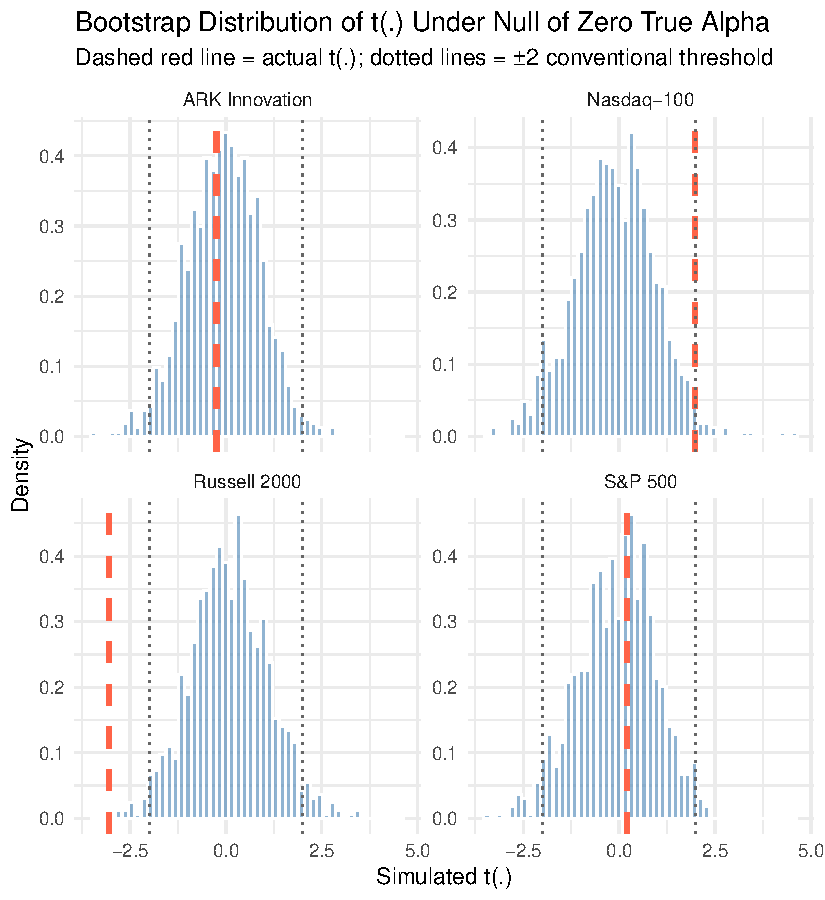
\includegraphics[keepaspectratio]{lecture02_skill_evaluation_files/figure-pdf/fig-bootstrap-1.pdf}}

}

\caption{\label{fig-bootstrap}Bootstrap distribution of t(α) vs.~actual
t(α) for selected ETFs}

\end{figure}%

\subsubsection{Step 5 --- Summarize Luck vs.~Skill
Evidence}\label{step-5-summarize-luck-vs.-skill-evidence}

\begin{Shaded}
\begin{Highlighting}[]
\NormalTok{pct\_actual }\SpecialCharTok{|\textgreater{}}
  \FunctionTok{arrange}\NormalTok{(}\FunctionTok{desc}\NormalTok{(pct\_beat)) }\SpecialCharTok{|\textgreater{}}
  \FunctionTok{select}\NormalTok{(name, t\_actual, pct\_beat) }\SpecialCharTok{|\textgreater{}}
  \FunctionTok{mutate}\NormalTok{(}
    \AttributeTok{interpretation =} \FunctionTok{case\_when}\NormalTok{(}
\NormalTok{      pct\_beat }\SpecialCharTok{\textgreater{}} \FloatTok{0.90} \SpecialCharTok{\textasciitilde{}} \StringTok{"Right{-}tail evidence of skill"}\NormalTok{,}
\NormalTok{      pct\_beat }\SpecialCharTok{\textless{}} \FloatTok{0.10} \SpecialCharTok{\textasciitilde{}} \StringTok{"Left{-}tail evidence of inferior performance"}\NormalTok{,}
      \ConstantTok{TRUE}            \SpecialCharTok{\textasciitilde{}} \StringTok{"Consistent with luck"}
\NormalTok{    )}
\NormalTok{  ) }\SpecialCharTok{|\textgreater{}}
  \FunctionTok{gt}\NormalTok{() }\SpecialCharTok{|\textgreater{}}
  \FunctionTok{fmt\_number}\NormalTok{(}\AttributeTok{columns =}\NormalTok{ t\_actual, }\AttributeTok{decimals =} \DecValTok{3}\NormalTok{) }\SpecialCharTok{|\textgreater{}}
  \CommentTok{\# Format pct\_beat for display but keep it NUMERIC in the underlying}
  \CommentTok{\# data, so the conditional fills below compare numbers to numbers.}
  \CommentTok{\# (Overwriting it with percent() would make it a character vector, and}
  \CommentTok{\#  "95.0\%" \textgreater{} 0.90 is a silent string comparison, not a numeric test.)}
  \FunctionTok{fmt\_percent}\NormalTok{(}\AttributeTok{columns =}\NormalTok{ pct\_beat, }\AttributeTok{decimals =} \DecValTok{1}\NormalTok{) }\SpecialCharTok{|\textgreater{}}
  \FunctionTok{cols\_label}\NormalTok{(}
    \AttributeTok{name           =} \StringTok{"ETF"}\NormalTok{,}
    \AttributeTok{t\_actual       =} \StringTok{"Actual t(α)"}\NormalTok{,}
    \AttributeTok{pct\_beat       =} \StringTok{"\% Simulations Below"}\NormalTok{,}
    \AttributeTok{interpretation =} \StringTok{"Inference"}
\NormalTok{  ) }\SpecialCharTok{|\textgreater{}}
  \FunctionTok{tab\_header}\NormalTok{(}
    \AttributeTok{title    =} \StringTok{"Bootstrap Inference: Luck vs. Skill"}\NormalTok{,}
    \AttributeTok{subtitle =} \FunctionTok{paste0}\NormalTok{(}\StringTok{"Based on "}\NormalTok{, scales}\SpecialCharTok{::}\FunctionTok{comma}\NormalTok{(n\_sim),}
                      \StringTok{" bootstrap simulations; joint monthly resampling"}\NormalTok{)}
\NormalTok{  ) }\SpecialCharTok{|\textgreater{}}
  \FunctionTok{tab\_footnote}\NormalTok{(}
    \AttributeTok{footnote  =} \StringTok{"Percent of simulations that produce t(α) below the actual value. Values \textgreater{}90\% suggest skill; \textless{}10\% suggest inferior performance."}\NormalTok{,}
    \AttributeTok{locations =} \FunctionTok{cells\_column\_labels}\NormalTok{(}\AttributeTok{columns =}\NormalTok{ pct\_beat)}
\NormalTok{  ) }\SpecialCharTok{|\textgreater{}}
  \FunctionTok{tab\_style}\NormalTok{(}
    \AttributeTok{style     =} \FunctionTok{cell\_fill}\NormalTok{(}\AttributeTok{color =} \StringTok{"\#e3f2fd"}\NormalTok{),}
    \AttributeTok{locations =} \FunctionTok{cells\_body}\NormalTok{(}\AttributeTok{rows =}\NormalTok{ pct\_beat }\SpecialCharTok{\textgreater{}} \FloatTok{0.90}\NormalTok{)}
\NormalTok{  ) }\SpecialCharTok{|\textgreater{}}
  \FunctionTok{tab\_style}\NormalTok{(}
    \AttributeTok{style     =} \FunctionTok{cell\_fill}\NormalTok{(}\AttributeTok{color =} \StringTok{"\#fce4ec"}\NormalTok{),}
    \AttributeTok{locations =} \FunctionTok{cells\_body}\NormalTok{(}\AttributeTok{rows =}\NormalTok{ pct\_beat }\SpecialCharTok{\textless{}} \FloatTok{0.10}\NormalTok{)}
\NormalTok{  )}
\end{Highlighting}
\end{Shaded}

\begin{table}

\caption{\label{tbl-bootstrap-summary}}

\centering{

\caption*{
{\fontsize{20}{25}\selectfont  Bootstrap Inference: Luck vs. Skill\fontsize{12}{15}\selectfont } \\ 
{\fontsize{14}{17}\selectfont  Based on 1,000 bootstrap simulations; joint monthly resampling\fontsize{12}{15}\selectfont }
} 
\fontsize{12.0pt}{14.0pt}\selectfont
\begin{tabular*}{\linewidth}{@{\extracolsep{\fill}}lrrl}
\toprule
ETF & Actual t(α) & \% Simulations Below\textsuperscript{\textit{1}} & Inference \\ 
\midrule\addlinespace[2.5pt]
{\cellcolor[HTML]{E3F2FD}{Nasdaq-100}} & {\cellcolor[HTML]{E3F2FD}{1.980}} & {\cellcolor[HTML]{E3F2FD}{98.2\%}} & {\cellcolor[HTML]{E3F2FD}{Right-tail evidence of skill}} \\ 
Vanguard Growth & 1.117 & 88.5\% & Consistent with luck \\ 
S\&P 500 & 0.214 & 58.8\% & Consistent with luck \\ 
Financials Sector & -0.088 & 46.1\% & Consistent with luck \\ 
ARK Innovation & -0.245 & 41.6\% & Consistent with luck \\ 
Energy Sector & -0.424 & 32.5\% & Consistent with luck \\ 
Vanguard Value & -0.768 & 21.4\% & Consistent with luck \\ 
{\cellcolor[HTML]{FCE4EC}{Real Estate (REIT)}} & {\cellcolor[HTML]{FCE4EC}{-1.306}} & {\cellcolor[HTML]{FCE4EC}{9.4\%}} & {\cellcolor[HTML]{FCE4EC}{Left-tail evidence of inferior performance}} \\ 
{\cellcolor[HTML]{FCE4EC}{Russell 1000 Value}} & {\cellcolor[HTML]{FCE4EC}{-2.327}} & {\cellcolor[HTML]{FCE4EC}{0.4\%}} & {\cellcolor[HTML]{FCE4EC}{Left-tail evidence of inferior performance}} \\ 
{\cellcolor[HTML]{FCE4EC}{Russell 2000}} & {\cellcolor[HTML]{FCE4EC}{-3.049}} & {\cellcolor[HTML]{FCE4EC}{0.0\%}} & {\cellcolor[HTML]{FCE4EC}{Left-tail evidence of inferior performance}} \\ 
\bottomrule
\end{tabular*}
\begin{minipage}{\linewidth}
\vspace{.05em}
\textsuperscript{\textit{1}}Percent of simulations that produce t(α) below the actual value. Values >90\% suggest skill; <10\% suggest inferior performance.\\
\end{minipage}

}

\end{table}%

\begin{tcolorbox}[enhanced jigsaw, arc=.35mm, bottomrule=.15mm, bottomtitle=1mm, breakable, colback=white, colbacktitle=quarto-callout-note-color!10!white, colframe=quarto-callout-note-color-frame, coltitle=black, left=2mm, leftrule=.75mm, opacityback=0, opacitybacktitle=0.6, rightrule=.15mm, title=\textcolor{quarto-callout-note-color}{\faInfo}\hspace{0.5em}{Note}, titlerule=0mm, toprule=.15mm, toptitle=1mm]

\textbf{Interpretation reminder}: Our ETF sample differs from Fama and
French (2010) in an important way. ETFs are passively managed (except
ARKK), so their ``alpha'' mainly reflects factor model misspecification
or expense ratios, not stock-picking skill. The bootstrap exercise here
is purely pedagogical. For genuine luck-vs.-skill inference, the
procedure should be applied to a large cross-section of \emph{actively
managed} open-end mutual funds.

\end{tcolorbox}

\subsubsection{Simulating the Value-Added
Measure}\label{simulating-the-value-added-measure}

To illustrate the Berk and Binsbergen (2015) approach, we compute a
simplified value-added measure for each ETF. We proxy AUM using the
ETF's market price × shares outstanding---not directly available via
\texttt{tidyquant}, so we demonstrate with hypothetical but plausible
AUM data.

\begin{Shaded}
\begin{Highlighting}[]
\CommentTok{\# Use hypothetical (approximate) average AUM for each ETF (in billions USD)}
\CommentTok{\# These are rough approximations for pedagogical illustration}
\NormalTok{aum\_proxy }\OtherTok{\textless{}{-}} \FunctionTok{tibble}\NormalTok{(}
  \AttributeTok{symbol =}\NormalTok{ etf\_tickers,}
  \AttributeTok{avg\_aum\_bn =} \FunctionTok{c}\NormalTok{(}\DecValTok{500}\NormalTok{, }\DecValTok{250}\NormalTok{, }\DecValTok{70}\NormalTok{, }\DecValTok{100}\NormalTok{, }\DecValTok{120}\NormalTok{, }\DecValTok{10}\NormalTok{, }\DecValTok{25}\NormalTok{, }\DecValTok{40}\NormalTok{, }\DecValTok{65}\NormalTok{, }\DecValTok{55}\NormalTok{)  }\CommentTok{\# approximate 2015{-}2024 avg AUM}
\NormalTok{)}

\CommentTok{\# Compute value added: AUM × gross excess return above RMRF benchmark}
\CommentTok{\# Here we use RMRF as the naive one{-}factor benchmark for illustration}
\NormalTok{value\_added }\OtherTok{\textless{}{-}}\NormalTok{ data\_merged }\SpecialCharTok{|\textgreater{}}
  \FunctionTok{left\_join}\NormalTok{(aum\_proxy, }\AttributeTok{by =} \StringTok{"symbol"}\NormalTok{) }\SpecialCharTok{|\textgreater{}}
  \FunctionTok{mutate}\NormalTok{(}
    \CommentTok{\# Simplified value added: AUM * (fund return {-} market return benchmark)}
    \CommentTok{\# In practice, BvB use the Vanguard multi{-}fund benchmark}
    \AttributeTok{gross\_excess\_vs\_mkt =}\NormalTok{ excess\_ret }\SpecialCharTok{{-}}\NormalTok{ RMRF,}
    \AttributeTok{value\_added\_mn =}\NormalTok{ avg\_aum\_bn }\SpecialCharTok{*} \DecValTok{1000} \SpecialCharTok{*}\NormalTok{ gross\_excess\_vs\_mkt  }\CommentTok{\# in $millions}
\NormalTok{  ) }\SpecialCharTok{|\textgreater{}}
  \FunctionTok{group\_by}\NormalTok{(symbol, name) }\SpecialCharTok{|\textgreater{}}
  \FunctionTok{summarise}\NormalTok{(}
    \AttributeTok{mean\_va\_ann  =} \FunctionTok{mean}\NormalTok{(value\_added\_mn, }\AttributeTok{na.rm =} \ConstantTok{TRUE}\NormalTok{) }\SpecialCharTok{*} \DecValTok{12}\NormalTok{,   }\CommentTok{\# annualized avg}
    \AttributeTok{mean\_alpha   =} \FunctionTok{mean}\NormalTok{(excess\_ret }\SpecialCharTok{{-}}\NormalTok{ RMRF, }\AttributeTok{na.rm =} \ConstantTok{TRUE}\NormalTok{) }\SpecialCharTok{*} \DecValTok{12}\NormalTok{,}
    \AttributeTok{avg\_aum\_bn   =} \FunctionTok{first}\NormalTok{(avg\_aum\_bn),}
    \AttributeTok{.groups      =} \StringTok{"drop"}
\NormalTok{  ) }\SpecialCharTok{|\textgreater{}}
  \FunctionTok{arrange}\NormalTok{(}\FunctionTok{desc}\NormalTok{(mean\_va\_ann))}

\NormalTok{value\_added }\SpecialCharTok{|\textgreater{}}
  \FunctionTok{gt}\NormalTok{() }\SpecialCharTok{|\textgreater{}}
  \FunctionTok{fmt\_number}\NormalTok{(}\AttributeTok{columns =} \FunctionTok{c}\NormalTok{(mean\_va\_ann, avg\_aum\_bn), }\AttributeTok{decimals =} \DecValTok{1}\NormalTok{) }\SpecialCharTok{|\textgreater{}}
  \FunctionTok{fmt\_percent}\NormalTok{(}\AttributeTok{columns =}\NormalTok{ mean\_alpha, }\AttributeTok{decimals =} \DecValTok{2}\NormalTok{) }\SpecialCharTok{|\textgreater{}}   \CommentTok{\# it is a return, not a count}
  \FunctionTok{cols\_label}\NormalTok{(}
    \AttributeTok{name        =} \StringTok{"ETF"}\NormalTok{,}
    \AttributeTok{mean\_va\_ann =} \StringTok{"Ann. Value Added ($M)"}\NormalTok{,}
    \AttributeTok{mean\_alpha  =} \StringTok{"Ann. Alpha (vs. Market)"}\NormalTok{,}
    \AttributeTok{avg\_aum\_bn  =} \StringTok{"Approx. AUM ($B)"}
\NormalTok{  ) }\SpecialCharTok{|\textgreater{}}
  \FunctionTok{tab\_header}\NormalTok{(}
    \AttributeTok{title    =} \StringTok{"Simplified Value{-}Added Illustration"}\NormalTok{,}
    \AttributeTok{subtitle =} \StringTok{"Pedagogical example: AUM × (fund return − market return)"}
\NormalTok{  ) }\SpecialCharTok{|\textgreater{}}
  \FunctionTok{tab\_footnote}\NormalTok{(}
    \AttributeTok{footnote  =} \StringTok{"AUM values are approximate. True BvB value added uses Vanguard fund benchmarks and precise historical AUM."}\NormalTok{,}
    \AttributeTok{locations =} \FunctionTok{cells\_title}\NormalTok{()}
\NormalTok{  )}
\end{Highlighting}
\end{Shaded}

\begin{table}
\caption*{
{\fontsize{20}{25}\selectfont  Simplified Value-Added Illustration\textsuperscript{\textit{1}}\fontsize{12}{15}\selectfont } \\ 
{\fontsize{14}{17}\selectfont  Pedagogical example: AUM × (fund return − market return)\textsuperscript{\textit{1}}\fontsize{12}{15}\selectfont }
} 
\fontsize{12.0pt}{14.0pt}\selectfont
\begin{tabular*}{\linewidth}{@{\extracolsep{\fill}}llrrr}
\toprule
symbol & ETF & Ann. Value Added (\$M) & Ann. Alpha (vs. Market) & Approx. AUM (\$B) \\ 
\midrule\addlinespace[2.5pt]
QQQ & Nasdaq-100 & 13,124.9 & 5.25\% & 250.0 \\ 
VUG & Vanguard Growth & 3,531.5 & 2.94\% & 120.0 \\ 
ARKK & ARK Innovation & 452.5 & 4.53\% & 10.0 \\ 
SPY & S\&P 500 & 187.9 & 0.04\% & 500.0 \\ 
XLF & Financials Sector & -298.9 & -0.75\% & 40.0 \\ 
XLE & Energy Sector & -1,087.0 & -4.35\% & 25.0 \\ 
IWD & Russell 1000 Value & -2,329.8 & -4.24\% & 55.0 \\ 
IWM & Russell 2000 & -2,638.1 & -3.77\% & 70.0 \\ 
VTV & Vanguard Value & -2,793.6 & -2.79\% & 100.0 \\ 
VNQ & Real Estate (REIT) & -4,602.6 & -7.08\% & 65.0 \\ 
\bottomrule
\end{tabular*}
\begin{minipage}{\linewidth}
\vspace{.05em}
\textsuperscript{\textit{1}}AUM values are approximate. True BvB value added uses Vanguard fund benchmarks and precise historical AUM.\\
\end{minipage}
\end{table}

\subsubsection{Illustrating the Power
Problem}\label{illustrating-the-power-problem}

The exercises above take the estimator's accuracy for granted. This one
checks it. Following (\textbf{andrikogiannopoulou2019?}), we build a
world where we \emph{know} the truth, run the FDR estimator on it, and
see what it reports.

The setup is deliberately generous to the FDR. We assume alphas are
estimated with no factor-model misspecification and no cross-sectional
correlation in residuals---both of which, in the paper, make matters
worse.

\begin{Shaded}
\begin{Highlighting}[]
\CommentTok{\# Parameters follow Andrikogiannopoulou \& Papakonstantinou (2019):}
\CommentTok{\# monthly residual SD of 0.021 in their baseline calibration, lambda = 0.5.}
\NormalTok{sigma\_e }\OtherTok{\textless{}{-}} \FloatTok{0.021}
\NormalTok{lambda  }\OtherTok{\textless{}{-}} \FloatTok{0.5}

\CommentTok{\# Simulate one cross{-}section of funds with KNOWN alphas, then apply the}
\CommentTok{\# FDR estimator of equation (2) and return its estimate of pi\^{}0.}
\NormalTok{fdr\_pi0 }\OtherTok{\textless{}{-}} \ControlFlowTok{function}\NormalTok{(n\_funds, T\_obs, pi0, pi\_neg, pi\_pos, alpha\_bar) \{}
\NormalTok{  se    }\OtherTok{\textless{}{-}}\NormalTok{ sigma\_e }\SpecialCharTok{/} \FunctionTok{sqrt}\NormalTok{(T\_obs)      }\CommentTok{\# SE of the monthly alpha estimate}
\NormalTok{  a\_m   }\OtherTok{\textless{}{-}}\NormalTok{ alpha\_bar }\SpecialCharTok{/} \DecValTok{12}             \CommentTok{\# annual alpha {-}\textgreater{} monthly}
\NormalTok{  truth }\OtherTok{\textless{}{-}} \FunctionTok{sample}\NormalTok{(}\FunctionTok{c}\NormalTok{(}\DecValTok{0}\NormalTok{, }\SpecialCharTok{{-}}\NormalTok{a\_m, a\_m), n\_funds, }\AttributeTok{replace =} \ConstantTok{TRUE}\NormalTok{,}
                  \AttributeTok{prob =} \FunctionTok{c}\NormalTok{(pi0, pi\_neg, pi\_pos))}
\NormalTok{  ahat  }\OtherTok{\textless{}{-}} \FunctionTok{rnorm}\NormalTok{(n\_funds, }\AttributeTok{mean =}\NormalTok{ truth, }\AttributeTok{sd =}\NormalTok{ se)}
\NormalTok{  pval  }\OtherTok{\textless{}{-}} \DecValTok{2} \SpecialCharTok{*}\NormalTok{ (}\DecValTok{1} \SpecialCharTok{{-}} \FunctionTok{pnorm}\NormalTok{(}\FunctionTok{abs}\NormalTok{(ahat }\SpecialCharTok{/}\NormalTok{ se)))}
  \FunctionTok{mean}\NormalTok{(pval }\SpecialCharTok{\textgreater{}}\NormalTok{ lambda) }\SpecialCharTok{/}\NormalTok{ (}\DecValTok{1} \SpecialCharTok{{-}}\NormalTok{ lambda)  }\CommentTok{\# equation (2)}
\NormalTok{\}}
\end{Highlighting}
\end{Shaded}

\begin{Shaded}
\begin{Highlighting}[]
\FunctionTok{set.seed}\NormalTok{(}\DecValTok{2019}\NormalTok{)}

\NormalTok{fdr\_grid }\OtherTok{\textless{}{-}} \FunctionTok{expand\_grid}\NormalTok{(}
  \AttributeTok{alpha\_bar =} \FunctionTok{c}\NormalTok{(}\FloatTok{0.010}\NormalTok{, }\FloatTok{0.020}\NormalTok{, }\FloatTok{0.035}\NormalTok{),}
  \AttributeTok{T\_obs     =} \FunctionTok{c}\NormalTok{(}\DecValTok{180}\NormalTok{, }\DecValTok{384}\NormalTok{)}
\NormalTok{) }\SpecialCharTok{|\textgreater{}}
  \FunctionTok{mutate}\NormalTok{(}
    \AttributeTok{pi0\_hat =} \FunctionTok{map2\_dbl}\NormalTok{(alpha\_bar, T\_obs, \textbackslash{}(a, t)}
      \FunctionTok{mean}\NormalTok{(}\FunctionTok{replicate}\NormalTok{(}\DecValTok{200}\NormalTok{, }\FunctionTok{fdr\_pi0}\NormalTok{(}\DecValTok{2000}\NormalTok{, t, }\FloatTok{0.75}\NormalTok{, }\FloatTok{0.23}\NormalTok{, }\FloatTok{0.02}\NormalTok{, a)))),}
    \AttributeTok{bias =}\NormalTok{ pi0\_hat }\SpecialCharTok{{-}} \FloatTok{0.75}
\NormalTok{  )}

\NormalTok{fdr\_grid }\SpecialCharTok{|\textgreater{}}
  \FunctionTok{mutate}\NormalTok{(}\AttributeTok{T\_lab =} \FunctionTok{if\_else}\NormalTok{(T\_obs }\SpecialCharTok{==} \DecValTok{180}\NormalTok{,}
                         \StringTok{"T = 180 (data median/mean)"}\NormalTok{,}
                         \StringTok{"T = 384 (BSW simulation)"}\NormalTok{)) }\SpecialCharTok{|\textgreater{}}
  \FunctionTok{select}\NormalTok{(T\_lab, alpha\_bar, pi0\_hat, bias) }\SpecialCharTok{|\textgreater{}}
  \FunctionTok{arrange}\NormalTok{(T\_lab, alpha\_bar) }\SpecialCharTok{|\textgreater{}}
  \FunctionTok{gt}\NormalTok{(}\AttributeTok{groupname\_col =} \StringTok{"T\_lab"}\NormalTok{) }\SpecialCharTok{|\textgreater{}}
  \FunctionTok{fmt\_percent}\NormalTok{(}\AttributeTok{columns =} \FunctionTok{c}\NormalTok{(alpha\_bar, pi0\_hat, bias), }\AttributeTok{decimals =} \DecValTok{1}\NormalTok{) }\SpecialCharTok{|\textgreater{}}
  \FunctionTok{cols\_label}\NormalTok{(}
    \AttributeTok{alpha\_bar =} \StringTok{"True |α| of nonzero funds (ann.)"}\NormalTok{,}
    \AttributeTok{pi0\_hat   =} \StringTok{"FDR estimate of π⁰"}\NormalTok{,}
    \AttributeTok{bias      =} \StringTok{"Bias (truth = 75\%)"}
\NormalTok{  ) }\SpecialCharTok{|\textgreater{}}
  \FunctionTok{tab\_header}\NormalTok{(}
    \AttributeTok{title    =} \StringTok{"The FDR Estimator Under Known Truth"}\NormalTok{,}
    \AttributeTok{subtitle =} \StringTok{"75\% zero{-}alpha, 23\% negative, 2\% positive — BSW\textquotesingle{}s own mix"}
\NormalTok{  ) }\SpecialCharTok{|\textgreater{}}
  \FunctionTok{tab\_style}\NormalTok{(}
    \AttributeTok{style     =} \FunctionTok{cell\_fill}\NormalTok{(}\AttributeTok{color =} \StringTok{"\#ffebee"}\NormalTok{),}
    \AttributeTok{locations =} \FunctionTok{cells\_body}\NormalTok{(}\AttributeTok{rows =}\NormalTok{ bias }\SpecialCharTok{\textgreater{}} \FloatTok{0.05}\NormalTok{)}
\NormalTok{  )}
\end{Highlighting}
\end{Shaded}

\begin{table}

\caption{\label{tbl-fdr-bias}FDR estimate of the zero-alpha proportion
when the truth is 75\%}

\centering{

\caption*{
{\fontsize{20}{25}\selectfont  The FDR Estimator Under Known Truth\fontsize{12}{15}\selectfont } \\ 
{\fontsize{14}{17}\selectfont  75\% zero-alpha, 23\% negative, 2\% positive — BSW's own mix\fontsize{12}{15}\selectfont }
} 
\fontsize{12.0pt}{14.0pt}\selectfont
\begin{tabular*}{\linewidth}{@{\extracolsep{\fill}}rrr}
\toprule
True |α| of nonzero funds (ann.) & FDR estimate of π⁰ & Bias (truth = 75\%) \\ 
\midrule\addlinespace[2.5pt]
\multicolumn{3}{l}{T = 180 (data median/mean)} \\[2.5pt] 
\midrule\addlinespace[2.5pt]
{\cellcolor[HTML]{FFEBEE}{1.0\%}} & {\cellcolor[HTML]{FFEBEE}{97.0\%}} & {\cellcolor[HTML]{FFEBEE}{22.0\%}} \\ 
{\cellcolor[HTML]{FFEBEE}{2.0\%}} & {\cellcolor[HTML]{FFEBEE}{90.4\%}} & {\cellcolor[HTML]{FFEBEE}{15.4\%}} \\ 
{\cellcolor[HTML]{FFEBEE}{3.5\%}} & {\cellcolor[HTML]{FFEBEE}{80.5\%}} & {\cellcolor[HTML]{FFEBEE}{5.5\%}} \\ 
\midrule\addlinespace[2.5pt]
\multicolumn{3}{l}{T = 384 (BSW simulation)} \\[2.5pt] 
\midrule\addlinespace[2.5pt]
{\cellcolor[HTML]{FFEBEE}{1.0\%}} & {\cellcolor[HTML]{FFEBEE}{94.0\%}} & {\cellcolor[HTML]{FFEBEE}{19.0\%}} \\ 
{\cellcolor[HTML]{FFEBEE}{2.0\%}} & {\cellcolor[HTML]{FFEBEE}{83.6\%}} & {\cellcolor[HTML]{FFEBEE}{8.6\%}} \\ 
3.5\% & 76.1\% & 1.1\% \\ 
\bottomrule
\end{tabular*}

}

\end{table}%

Read the bottom row of each block first. With \(T = 384\) and alphas of
±3.5\% per year---BSW's simulation design---the FDR recovers a \(\pi^0\)
of about 76\% against a truth of 75\%. The estimator looks excellent,
which is exactly what BSW reported.

Now read upward. Holding everything else fixed and shrinking the true
alpha to ±1\% per year, the same estimator reports that roughly 94\% of
funds have zero alpha. Nothing changed about the method; only the world
it was applied to.

\begin{Shaded}
\begin{Highlighting}[]
\NormalTok{misclass }\OtherTok{\textless{}{-}} \ControlFlowTok{function}\NormalTok{(alpha\_bar, T\_obs) \{}
\NormalTok{  se }\OtherTok{\textless{}{-}}\NormalTok{ sigma\_e }\SpecialCharTok{/} \FunctionTok{sqrt}\NormalTok{(T\_obs)}
  \CommentTok{\# P(p{-}value \textgreater{} lambda) for a fund whose true alpha is alpha\_bar,}
  \CommentTok{\# scaled by 1/(1{-}lambda) because equation (2) extrapolates.}
\NormalTok{  p\_above }\OtherTok{\textless{}{-}} \FunctionTok{pnorm}\NormalTok{(}\FunctionTok{qnorm}\NormalTok{(}\DecValTok{1} \SpecialCharTok{{-}}\NormalTok{ lambda }\SpecialCharTok{/} \DecValTok{2}\NormalTok{) }\SpecialCharTok{{-}}\NormalTok{ (alpha\_bar }\SpecialCharTok{/} \DecValTok{12}\NormalTok{) }\SpecialCharTok{/}\NormalTok{ se)}
  \FunctionTok{pmin}\NormalTok{(}\DecValTok{1}\NormalTok{, p\_above }\SpecialCharTok{/}\NormalTok{ (}\DecValTok{1} \SpecialCharTok{{-}}\NormalTok{ lambda))}
\NormalTok{\}}

\FunctionTok{expand\_grid}\NormalTok{(}
  \AttributeTok{alpha\_bar =} \FunctionTok{seq}\NormalTok{(}\FloatTok{0.005}\NormalTok{, }\FloatTok{0.05}\NormalTok{, }\AttributeTok{by =} \FloatTok{0.001}\NormalTok{),}
  \AttributeTok{T\_obs     =} \FunctionTok{c}\NormalTok{(}\DecValTok{120}\NormalTok{, }\DecValTok{180}\NormalTok{, }\DecValTok{384}\NormalTok{)}
\NormalTok{) }\SpecialCharTok{|\textgreater{}}
  \FunctionTok{mutate}\NormalTok{(}
    \AttributeTok{rate  =} \FunctionTok{misclass}\NormalTok{(alpha\_bar, T\_obs),}
    \AttributeTok{T\_lab =} \FunctionTok{factor}\NormalTok{(T\_obs, }\AttributeTok{levels =} \FunctionTok{c}\NormalTok{(}\DecValTok{120}\NormalTok{, }\DecValTok{180}\NormalTok{, }\DecValTok{384}\NormalTok{),}
                   \AttributeTok{labels =} \FunctionTok{c}\NormalTok{(}\StringTok{"T = 120"}\NormalTok{, }\StringTok{"T = 180 (realistic)"}\NormalTok{, }\StringTok{"T = 384"}\NormalTok{))}
\NormalTok{  ) }\SpecialCharTok{|\textgreater{}}
  \FunctionTok{ggplot}\NormalTok{(}\FunctionTok{aes}\NormalTok{(alpha\_bar, rate, }\AttributeTok{color =}\NormalTok{ T\_lab)) }\SpecialCharTok{+}
  \FunctionTok{geom\_line}\NormalTok{(}\AttributeTok{linewidth =} \FloatTok{0.8}\NormalTok{) }\SpecialCharTok{+}
  \FunctionTok{geom\_vline}\NormalTok{(}\AttributeTok{xintercept =} \FunctionTok{c}\NormalTok{(}\FloatTok{0.01}\NormalTok{, }\FloatTok{0.02}\NormalTok{), }\AttributeTok{linetype =} \StringTok{"dotted"}\NormalTok{, }\AttributeTok{color =} \StringTok{"grey40"}\NormalTok{) }\SpecialCharTok{+}
  \FunctionTok{annotate}\NormalTok{(}\StringTok{"text"}\NormalTok{, }\AttributeTok{x =} \FloatTok{0.0205}\NormalTok{, }\AttributeTok{y =} \FloatTok{0.05}\NormalTok{, }\AttributeTok{hjust =} \DecValTok{0}\NormalTok{, }\AttributeTok{size =} \DecValTok{3}\NormalTok{,}
           \AttributeTok{label =} \StringTok{"±1\% and ±2\% per year"}\NormalTok{) }\SpecialCharTok{+}
  \FunctionTok{scale\_x\_continuous}\NormalTok{(}\AttributeTok{labels =} \FunctionTok{percent\_format}\NormalTok{()) }\SpecialCharTok{+}
  \FunctionTok{scale\_y\_continuous}\NormalTok{(}\AttributeTok{labels =} \FunctionTok{percent\_format}\NormalTok{(), }\AttributeTok{limits =} \FunctionTok{c}\NormalTok{(}\DecValTok{0}\NormalTok{, }\DecValTok{1}\NormalTok{)) }\SpecialCharTok{+}
  \FunctionTok{labs}\NormalTok{(}
    \AttributeTok{x =} \StringTok{"True annual alpha of a nonzero{-}alpha fund"}\NormalTok{,}
    \AttributeTok{y =} \StringTok{"Probability of being counted as zero{-}alpha"}\NormalTok{,}
    \AttributeTok{color =} \ConstantTok{NULL}\NormalTok{,}
    \AttributeTok{title =} \StringTok{"Where the FDR loses skilled managers"}\NormalTok{,}
    \AttributeTok{subtitle =} \StringTok{"Economically large alphas are invisible at realistic sample lengths"}
\NormalTok{  ) }\SpecialCharTok{+}
  \FunctionTok{theme\_minimal}\NormalTok{() }\SpecialCharTok{+}
  \FunctionTok{theme}\NormalTok{(}\AttributeTok{legend.position =} \StringTok{"bottom"}\NormalTok{)}
\end{Highlighting}
\end{Shaded}

\begin{figure}[H]

\centering{

\pandocbounded{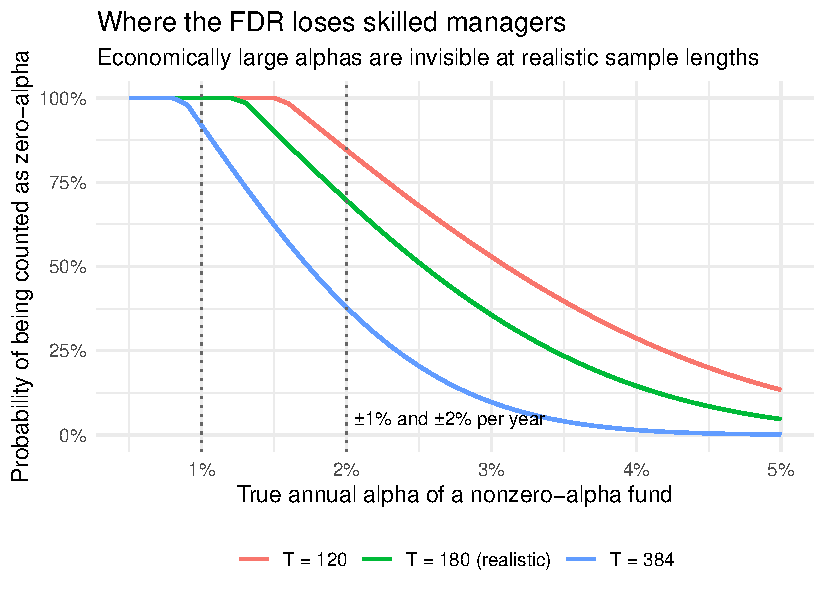
\includegraphics[keepaspectratio]{lecture02_skill_evaluation_files/figure-pdf/fig-misclass-1.pdf}}

}

\caption{\label{fig-misclass}Share of genuinely nonzero-alpha funds that
the FDR classifies as zero-alpha}

\end{figure}%

\begin{tcolorbox}[enhanced jigsaw, arc=.35mm, bottomrule=.15mm, bottomtitle=1mm, breakable, colback=white, colbacktitle=quarto-callout-warning-color!10!white, colframe=quarto-callout-warning-color-frame, coltitle=black, left=2mm, leftrule=.75mm, opacityback=0, opacitybacktitle=0.6, rightrule=.15mm, title=\textcolor{quarto-callout-warning-color}{\faExclamationTriangle}\hspace{0.5em}{How closely does this match the paper?}, titlerule=0mm, toprule=.15mm, toptitle=1mm]

Reasonably, but not exactly, and the gap is worth understanding.

Our simplified version draws \(\hat\alpha\) directly from a normal
rather than estimating it from a factor regression, and it fixes
\(\lambda = 0.5\) where (\textbf{andrikogiannopoulou2019?}) select
\(\lambda\) optimally by bootstrap and average over 1,000 repetitions.
It reproduces their central case closely---at \(T = 384\) with ±3.5\%
alphas we get \(\hat\pi^0 \approx 76\%\) against their reported
76.3\%---but our misclassification rates for small alphas run somewhat
higher than their simulated 90\% and 65\% figures.

Treat the exact numbers here as illustrative and the paper's as
authoritative. The mechanism, the sign of the bias, and its order of
magnitude are what this exercise is for. The fact that a
back-of-envelope reproduces the qualitative result is itself the point:
the bias is not subtle, and anyone could have checked.

\end{tcolorbox}

\begin{center}\rule{0.5\linewidth}{0.5pt}\end{center}

\subsection{11. Summary Statistics and
Comparison}\label{summary-statistics-and-comparison}

\begin{Shaded}
\begin{Highlighting}[]
\CommentTok{\# Combine Carhart results with bootstrap pct and AUM}
\NormalTok{final\_tbl }\OtherTok{\textless{}{-}}\NormalTok{ carhart\_base }\SpecialCharTok{|\textgreater{}}
  \FunctionTok{select}\NormalTok{(name, alpha\_ann, alpha\_statistic, b\_mkt\_estimate) }\SpecialCharTok{|\textgreater{}}
  \FunctionTok{left\_join}\NormalTok{(pct\_actual }\SpecialCharTok{|\textgreater{}} \FunctionTok{select}\NormalTok{(name, pct\_beat), }\AttributeTok{by =} \StringTok{"name"}\NormalTok{) }\SpecialCharTok{|\textgreater{}}
  \FunctionTok{arrange}\NormalTok{(}\FunctionTok{desc}\NormalTok{(alpha\_ann))}

\NormalTok{final\_tbl }\SpecialCharTok{|\textgreater{}}
  \FunctionTok{gt}\NormalTok{() }\SpecialCharTok{|\textgreater{}}
  \FunctionTok{fmt\_number}\NormalTok{(}\AttributeTok{columns =} \FunctionTok{c}\NormalTok{(alpha\_ann, alpha\_statistic, b\_mkt\_estimate), }\AttributeTok{decimals =} \DecValTok{3}\NormalTok{) }\SpecialCharTok{|\textgreater{}}
  \FunctionTok{fmt\_percent}\NormalTok{(}\AttributeTok{columns =}\NormalTok{ pct\_beat, }\AttributeTok{decimals =} \DecValTok{1}\NormalTok{) }\SpecialCharTok{|\textgreater{}}
  \FunctionTok{cols\_label}\NormalTok{(}
    \AttributeTok{name             =} \StringTok{"ETF"}\NormalTok{,}
    \AttributeTok{alpha\_ann        =} \StringTok{"Carhart α (Ann.)"}\NormalTok{,}
    \AttributeTok{alpha\_statistic  =} \StringTok{"t(α)"}\NormalTok{,}
    \AttributeTok{b\_mkt\_estimate   =} \StringTok{"β(MKT)"}\NormalTok{,}
    \AttributeTok{pct\_beat         =} \StringTok{"Bootstrap \%ile"}
\NormalTok{  ) }\SpecialCharTok{|\textgreater{}}
  \FunctionTok{tab\_header}\NormalTok{(}
    \AttributeTok{title    =} \StringTok{"Fund Performance Summary with Bootstrap Inference"}\NormalTok{,}
    \AttributeTok{subtitle =} \StringTok{"Bootstrap \%ile = fraction of simulations with t(α) below actual"}
\NormalTok{  ) }\SpecialCharTok{|\textgreater{}}
  \FunctionTok{data\_color}\NormalTok{(}
    \AttributeTok{columns =}\NormalTok{ alpha\_ann,}
    \AttributeTok{fn =}\NormalTok{ scales}\SpecialCharTok{::}\FunctionTok{col\_numeric}\NormalTok{(}
      \AttributeTok{palette =} \FunctionTok{c}\NormalTok{(}\StringTok{"tomato"}\NormalTok{, }\StringTok{"white"}\NormalTok{, }\StringTok{"steelblue"}\NormalTok{),}
      \AttributeTok{domain  =} \ConstantTok{NULL}
\NormalTok{    )}
\NormalTok{  )}
\end{Highlighting}
\end{Shaded}

\begin{table}

\caption{\label{tbl-final-summary}}

\centering{

\caption*{
{\fontsize{20}{25}\selectfont  Fund Performance Summary with Bootstrap Inference\fontsize{12}{15}\selectfont } \\ 
{\fontsize{14}{17}\selectfont  Bootstrap \%ile = fraction of simulations with t(α) below actual\fontsize{12}{15}\selectfont }
} 
\fontsize{12.0pt}{14.0pt}\selectfont
\begin{tabular*}{\linewidth}{@{\extracolsep{\fill}}lrrrr}
\toprule
ETF & Carhart α (Ann.) & t(α) & β(MKT) & Bootstrap \%ile \\ 
\midrule\addlinespace[2.5pt]
Nasdaq-100 & {\cellcolor[HTML]{4682B4}{\textcolor[HTML]{FFFFFF}{0.033}}} & 1.980 & 1.082 & 98.2\% \\ 
Vanguard Growth & {\cellcolor[HTML]{A5BDD9}{\textcolor[HTML]{000000}{0.012}}} & 1.117 & 1.074 & 88.5\% \\ 
S\&P 500 & {\cellcolor[HTML]{D4DFED}{\textcolor[HTML]{000000}{0.001}}} & 0.214 & 0.981 & 58.8\% \\ 
Financials Sector & {\cellcolor[HTML]{DFE7F1}{\textcolor[HTML]{000000}{-0.002}}} & -0.088 & 1.061 & 46.1\% \\ 
Vanguard Value & {\cellcolor[HTML]{FCFCFE}{\textcolor[HTML]{000000}{-0.009}}} & -0.768 & 0.886 & 21.4\% \\ 
ARK Innovation & {\cellcolor[HTML]{FFEEE9}{\textcolor[HTML]{000000}{-0.014}}} & -0.245 & 1.518 & 41.6\% \\ 
Russell 2000 & {\cellcolor[HTML]{FFCCBD}{\textcolor[HTML]{000000}{-0.024}}} & -3.049 & 1.032 & 0.0\% \\ 
Energy Sector & {\cellcolor[HTML]{FFCCBD}{\textcolor[HTML]{000000}{-0.024}}} & -0.424 & 1.093 & 32.5\% \\ 
Russell 1000 Value & {\cellcolor[HTML]{FFCABA}{\textcolor[HTML]{000000}{-0.025}}} & -2.327 & 0.915 & 0.4\% \\ 
Real Estate (REIT) & {\cellcolor[HTML]{FF6347}{\textcolor[HTML]{FFFFFF}{-0.052}}} & -1.306 & 0.857 & 9.4\% \\ 
\bottomrule
\end{tabular*}

}

\end{table}%

\begin{center}\rule{0.5\linewidth}{0.5pt}\end{center}

\subsection{12. Key Takeaways}\label{key-takeaways}

\begin{enumerate}
\def\labelenumi{\arabic{enumi}.}
\item
  \textbf{Equilibrium accounting constrains aggregate performance} (Fama
  and French 2010). Before costs, aggregate active management must have
  zero alpha. After costs, it must be negative. This is arithmetic, not
  an empirical finding.
\item
  \textbf{The bootstrap simulation is the right tool} for separating
  luck from skill in large fund cross-sections. Standard t-tests fail
  due to multiple comparisons and cross-fund correlation. Joint
  resampling of months preserves the correlation structure of fund
  returns.
\item
  \textbf{Few funds cover costs on net returns} (Fama and French 2010).
  The cross-section of t(α) for net returns is almost entirely to the
  left of the simulated null distribution. Skill is detectable only in
  the extreme right tail (≥97th percentile) and even then the evidence
  is mixed.
\item
  \textbf{Skill exists in gross returns}, with true alpha dispersion of
  roughly ±1.25\% per year. But this barely covers average expense
  ratios of 1\%.
\item
  \textbf{The FDR estimate that ``75\% of funds have zero alpha'' does
  not survive scrutiny} (\textbf{andrikogiannopoulou2019?}). At
  realistic sample lengths the methodology misclassifies 65\% of funds
  with alphas of ±2\% per year, and 90\% of those with ±1\%. The bias is
  upward in \(\pi^0\) by construction, because equation (2) extrapolates
  every failure to reject.
\item
  \textbf{Low power is not a caveat; it can invert the conclusion.}
  Under a data-generating process calibrated to Fama and French's own
  estimate of alpha dispersion---where only 1\% of funds truly have zero
  alpha---the FDR reports 70\% zero-alpha funds. An estimator that
  returns BSW's answer whether or not BSW's world obtains is not
  evidence for that world, and therefore not evidence for Berk and Green
  (2004) either.
\item
  \textbf{Power comes from} \(T\), not \(N\). Adding funds does not
  improve the FDR estimator at all; only lengthening each fund's return
  history does, and convergence is so slow that even 200 years of
  monthly data would be insufficient. This generalizes well beyond fund
  performance.
\item
  \textbf{Alpha is the wrong measure of skill} (Berk and Binsbergen
  2015). Under standard neoclassical assumptions, neither net alpha
  (driven to zero by competition) nor gross alpha (equals the manager's
  chosen fee) measures skill. Value added---AUM times gross excess
  return---is the correct measure.
\item
  \textbf{The average fund adds \$3.2 million per year} in dollar terms
  (Berk and Binsbergen 2015). Skill is widespread but concentrated among
  large funds. Cross-sectional differences in skill persist for up to 10
  years---far longer than persistence in alpha.
\item
  \textbf{Investors appear to identify skill}: managerial compensation
  (AUM × fee) predicts future value added. Capital flows to skilled
  managers, consistent with Berk and Green (2004).
\item
  \textbf{Skilled managers capture all rents}: net alpha to investors is
  approximately zero even for the best funds. There is no free lunch in
  active management---the benefit of skill accrues to the manager, not
  the investor.
\end{enumerate}

\begin{center}\rule{0.5\linewidth}{0.5pt}\end{center}

\subsection{Discussion Questions}\label{discussion-questions}

\begin{enumerate}
\def\labelenumi{\arabic{enumi}.}
\item
  Fama and French (2010) find that the VW portfolio of active funds has
  a net alpha of approximately −1\% per year. Is this evidence that
  active managers \emph{lack} skill, or evidence that \emph{investors}
  rationally drive net alphas to zero? How would you distinguish between
  these two interpretations empirically?
\item
  Berk and Binsbergen (2015) argue that gross alpha is not a valid
  measure of skill because it equals the fee the manager charges. Does
  this imply that a manager who charges 2\% in fees is more skilled than
  one who charges 0.5\%? What does the theory actually predict about the
  relationship between fees and skill?
\item
  The Fama and French (2010) bootstrap preserves cross-correlation by
  jointly sampling months for all funds. Why is this important? What
  would happen to the simulation results if each fund's months were
  sampled independently?
\item
  Berk and Binsbergen (2015) use Vanguard index funds rather than FFC
  factors as the benchmark. Their Table 2 shows that HML and UMD have
  significant positive alpha relative to Vanguard funds. What does this
  imply about alpha estimates computed using FFC factors for the early
  part of the sample?
\item
  Suppose a fund manager has a true annual alpha of 2\% and manages
  \$100 million. Under the Berk-Green (2004) model, what happens to the
  fund's alpha and AUM over time as investors observe the fund's
  performance? Is this story consistent with Berk and Binsbergen
  (2015)'s finding that value-added persistence lasts 10 years?
\item
  Fama and French (2010) find that the CAPM (single-factor) bootstrap
  produces much stronger apparent evidence of skill than the four-factor
  bootstrap. Why does adding size, value, and momentum factors to the
  benchmark reduce the apparent evidence of skill? What does this tell
  you about the source of ``alpha'' in a CAPM regression?
\item
  Write down the assumption behind equation (2) in words, then state
  precisely when it fails. (\textbf{andrikogiannopoulou2019?}) show that
  the resulting bias in \(\hat\pi^0\) is always \emph{upward}. Explain
  why the bias cannot go the other way, and why the factor
  \(1/(1-\lambda)\) makes it worse rather than better.
\item
  (\textbf{andrikogiannopoulou2019?}) find that increasing the number of
  funds \(N\) does not reduce the FDR estimator's bias, while increasing
  the number of observations per fund \(T\) does. Explain the asymmetry.
  Then consider: does the Fama and French (2010) bootstrap suffer from
  the same problem? Which features of the bootstrap make it more or less
  vulnerable than the FDR, and does it escape the low-power critique
  entirely?
\item
  Suppose you are refereeing a paper that applies the FDR methodology to
  a panel of 3,000 hedge funds with an average of 48 monthly return
  observations each. Using the reasoning in
  (\textbf{andrikogiannopoulou2019?}), what would you ask the authors to
  demonstrate before you would believe their estimated proportions? Be
  specific about the simulation you would request.
\end{enumerate}

\begin{center}\rule{0.5\linewidth}{0.5pt}\end{center}

\subsection{References}\label{references}

\protect\phantomsection\label{refs}
\begin{CSLReferences}{1}{1}
\bibitem[\citeproctext]{ref-berkvanBinsbergen2015}
Berk, Jonathan B., and Jules H. van Binsbergen. 2015. {``Measuring Skill
in the Mutual Fund Industry.''} \emph{Journal of Financial Economics}
118 (1): 1--20. \url{https://doi.org/10.1016/j.jfineco.2015.05.002}.

\bibitem[\citeproctext]{ref-berkgreen2004}
Berk, Jonathan B., and Richard C. Green. 2004. {``Mutual Fund Flows and
Performance in Rational Markets.''} \emph{Journal of Political Economy}
112 (6): 1269--95. \url{https://doi.org/10.1086/424739}.

\bibitem[\citeproctext]{ref-carhart1997}
Carhart, Mark M. 1997. {``On Persistence in Mutual Fund Performance.''}
\emph{Journal of Finance} 52 (1): 57--82.

\bibitem[\citeproctext]{ref-fama2010}
Fama, Eugene F., and Kenneth R. French. 2010. {``Luck Versus Skill in
the Cross-Section of Mutual Fund Returns.''} \emph{Journal of Finance}
65 (5): 1915--47.
\url{https://doi.org/10.1111/j.1540-6261.2010.01598.x}.

\bibitem[\citeproctext]{ref-kosowski2006}
Kosowski, Robert, Allan Timmermann, Russ Wermers, and Hal White. 2006.
{``Can Mutual Fund {`Stars'} Really Pick Stocks? New Evidence from a
Bootstrap Analysis.''} \emph{Journal of Finance} 61 (6): 2551--95.
\url{https://doi.org/10.1111/j.1540-6261.2006.01015.x}.

\bibitem[\citeproctext]{ref-sharpe1991}
Sharpe, William F. 1991. {``The Arithmetic of Active Management.''}
\emph{Financial Analysts Journal} 47 (1): 7--9.

\bibitem[\citeproctext]{ref-wermers2011}
Wermers, Russ. 2011. {``Performance Measurement of Mutual Funds, Hedge
Funds, and Institutional Accounts.''} \emph{Annual Review of Financial
Economics} 3: 537--74.

\end{CSLReferences}




\end{document}
